%!TEX root = ../thesis.tex
%*******************************************************************************
%****************************** Third Chapter **********************************
%*******************************************************************************

% **************************** Define Graphics Path **************************
\ifpdf
    \graphicspath{{Chapter3/Figs/Raster/}{Chapter3/Figs/PDF/}{Chapter3/Figs/}}
\else
    \graphicspath{{Chapter3/Figs/Vector/}{Chapter3/Figs/}}
\fi

%*******************************************************************************
%****************************** Second Chapter *********************************
%*******************************************************************************

\chapter{The RMON and VIDARR Detectors}\label{Chp:ThePrototypeDetector}

\section{Technology And Results Of RMON}
This thesis will cover two distinct versions of the detector. The original prototype detector was repurposed technology from the T2K ND280 ECal \cite{Allan_2013} and an upgraded version that uses the same basic materials in the detector but upgraded electronics and containment which will be referred to as the VIDARR detector. The rest of this section will focus on the prototype detector.
\\\\As it is the basis for the other detectors a quick overview of the T2K ND280 ECal will be required. The ND280 is a series of detectors from the neutrino oscillation experiment T2K which relies on a $\nu_\mu$ beam entering the detector shown in figure \ref{fig:nd280Fig}. This detector was comprised of several different detectors including time projection chambers (TPCs) and fine-grained detectors (FGDs) and electromagnetic calorimeters (ECals) \cite{Allan_2013}. The ECals are of particular interest as they are the basis for the prototype and VIDARR detectors. 

\begin{figure}[!h]
 \centering
 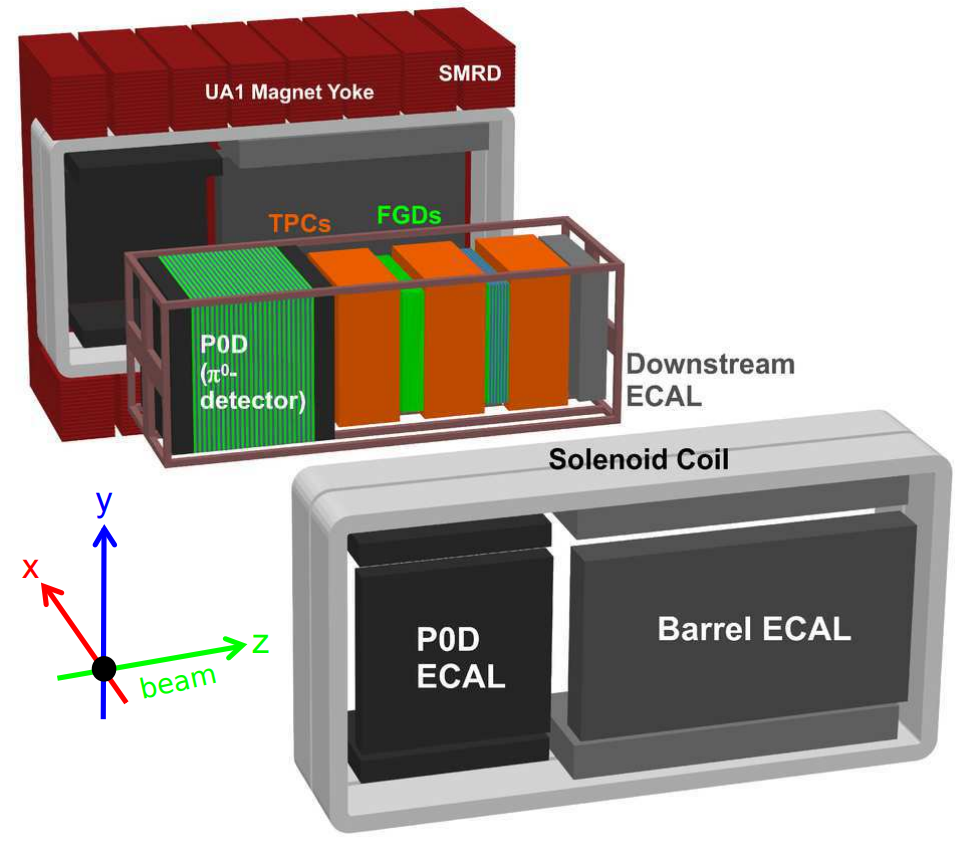
\includegraphics[width=\linewidth/2]{Chapter2/Figs/Raster/ND280Fig.png} 
 \captionof{figure}{Diagram of the ND280 detector. From \cite{Allan_2013}} %~can be used as a kind of place holder in latex
 \label{fig:nd280Fig}
\end{figure}

The T2K Ecals were made from plastic scintillating bars measuring 4\,cm by 1\,cm with varying lengths arranged in alternating layers at 90 degrees to each other \cite{Allan_2013}. Wavelength shifting (WLS) fibres were placed in the centre of the scintillating bars which shift the wavelength from blue to green \cite{Allan_2013}. These wavelength shifting fibres are then connected to multi-pixel photon counters (MPPCs) which are the instruments that read out the signal. This signal is then read in by Trip-T front-end electronic boards (TFBs) which then splits the signal into different cycles each containing 1.5 microseconds of information. All of this is shared by the prototype detector. 
\\\\However, a crucial difference between the ECals of the ND280 and the prototype detector is that the (ECals) had a layer of lead in between each of the plastic scintillating layers \cite{Allan_2013}. In the prototype, this has been replaced with a layer of gadolinium sulphate so that neutrons produced in IBD (equation \ref{inverse_beta_decay}) are captured. The prototype was also designed to fit inside of a shipping container each bar having a length of 152\,cm and the whole detector measuring 152\,cm by 152\,cm with 49 layers of plastic scintillating bars giving a height of 49\,cm and a total of 1862 bars. The electronic systems were also adapted from the T2K ECal. However, they were altered such that they were triggered from a neutron-induced gadolinium cascade from IBD. There were 23 cycles numbered from 0 -- 22 with 0 -- 17 cycles being considered "prompt" and cycle 18 being the trigger cycle. Cycles 19 -- 22 were left alone so that they could be compared in case time-dependent issues arose from the altered system. As will be discussed later in chapter \ref{chp:cosmicMuonTomography} these cycles were used to diagnose a time dependant issue with the cosmic $\mu$ data set.
\\The overall structure for the detector can be seen in figure \ref{fig:vidarrDiagram} where the orientation of the segments and how the WLS fibres shift protrude out of the ends is shown. In-between the layers of plastic there are layers of Gadolinium which absorb the neutrons from inverse $\beta$ decay shown in figure \ref{fig:inverse_beta_diagram}. The $\Bar{\nu_e}$ will be absorbed by a proton and decay into a $e^+$ and a neutron as shown in figure \ref{fig:inverse_beta_diagram}. The e$^+$ will decay producing two $\gamma$ rays which could be useful in distinguishing the e$^+$ from the general e$^-$ background. The neutron shown in figure \ref{fig:inverse_beta_diagram} is absorbed by the Gadolinium sheets in the detector which then causes an 8\,MeV $\gamma$ cascade which will be expanded upon in section \ref{sec:GEANT4Simulation_modellingGadolinium}.  

\begin{figure}[!h]
 \centering
 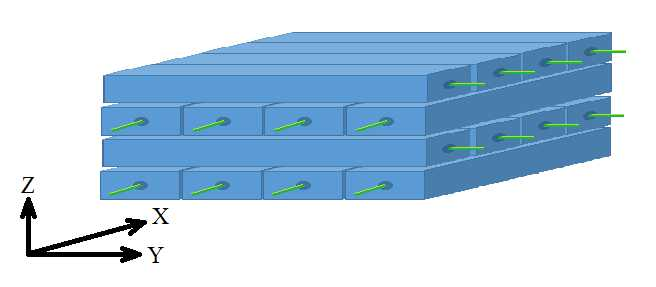
\includegraphics[width=0.8\linewidth]{Chapter2/Figs/Raster/VIDARR_diagram.jpeg} 
 \captionof{figure}{A cutaway diagram showing the structure of the VIDARR detector. The segments are 4\,cm wide by 152\,cm long by 1\,cm tall. The Gadolinium sheets in-between the VIDARR segments are not shown. (diagram created by George Holt fellow VIDARR collaborator).} 
 \label{fig:vidarrDiagram}
\end{figure}

\begin{figure}[!h]
 \centering
 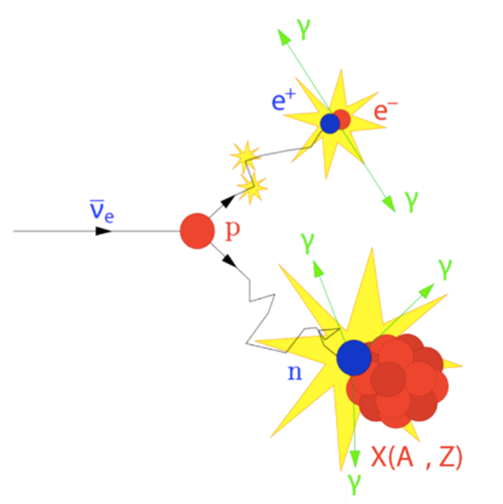
\includegraphics[width =0.7\linewidth]{Chapter2/Figs/Raster/inverse_beta_diagram.png}
 \captionof{figure}{A diagram of inverse $\beta$ decay 
 (equation \ref{inverse_beta_decay}). The neutrons random walk means it will take some time before it is detected the positron emission is prompt. From \cite{ibdPictureLink}.} 
 \label{fig:inverse_beta_diagram}
\end{figure}

The original detector was deployed at the Wylfa power station in Anglesey Wales for an 18-month period. This run proved successful in measuring the power from the reactor to within good agreement of the measured reactor flux. Figure \ref{fig:prototypeMeasumentFlux} compares the measured $\bar{\nu_e}$ flux with the reported power output and shows how good the agreement is. A measured anti-neutrino rate of 172.1 $\pm$ 4.6 candidates per day is observed when the reactor is off and 203.7 $\pm$ 19.6 when the reactor is on \cite{Carroll_2018}. Unfortunately due to cooling issues with the prototype detector the reactor shutdown was not observed. This is one of the main motivating factors behind the upgrade of the detector as the first generation MPPCs and repurposed electronics were susceptible to high levels of noise if the temperature was not carefully controlled. 
\begin{figure}[!h]
 \centering
 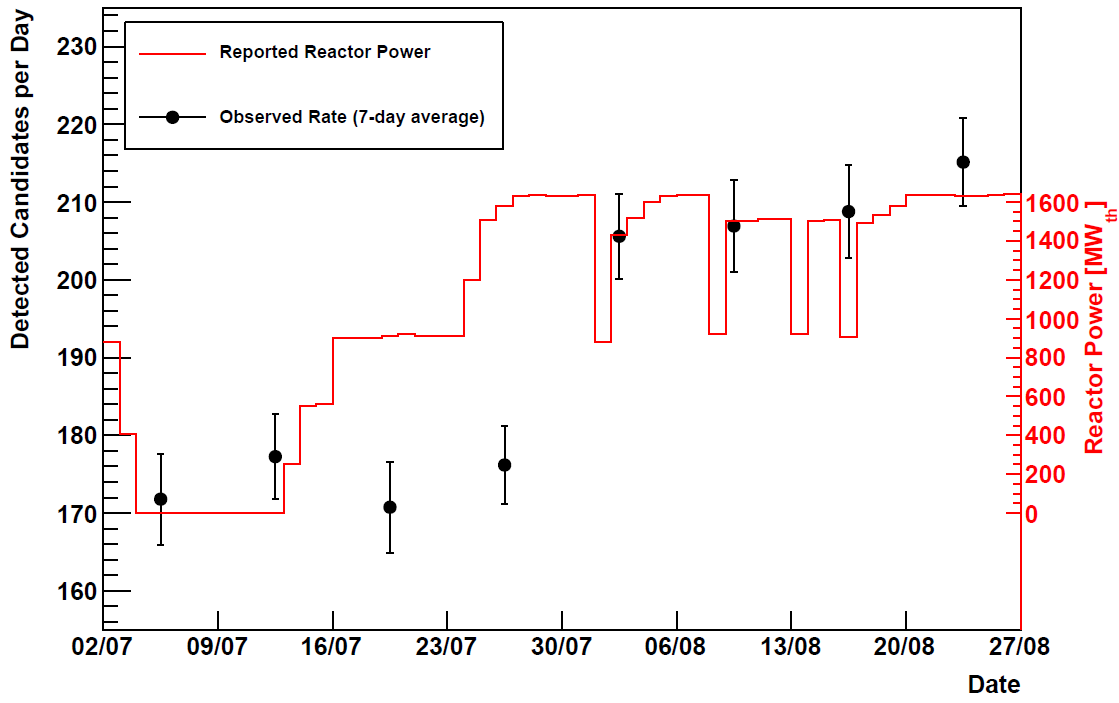
\includegraphics[width=0.90\linewidth]{Chapter2/Figs/Raster/prototypeMeasureOnFig.png} 
 \captionof{figure}{Measured anti-neutrino flux compared to the power generation from the Wylfa power station. From \cite{Carroll_2018}} %~can be used as a kind of place holder in latex
 \label{fig:prototypeMeasumentFlux}
\end{figure}

\section{Background At Reactor Sites}
The PROSPECT experiment has done a  study looking into the background at two research reactor locations difference between the National Bureau of Standards Reactor (NBSR) at NIST and the High Flux Isotope Reactor (HFIR) at ORNL \cite{Ashenfelter_2016}. Another site was considered by the PROSPECT the ATR at INL but the increased altitude of that site leads to a significantly higher cosmogenic neutron flux \cite{Ashenfelter_2016}. An example of how reactors affect the background can be seen in figure \ref{fig:Prospect_NSBR_gammaSpec} which shows how the $\gamma$ spectrum varies when the NBSR is on and off, it shows how the spectrum between 3\,MeV -- 9\,MeV is mostly dominated by reactor noise. Another component is neutron measurements caused by the reactor which is shown in figure \ref{fig:prospectNeutronMap} for thermal neutrons which are an issue for $\bar{\nu_e}$ detectors but should be somewhat negated through robust e$^+$ identification and accurate double coincident measurements. Another more important background is fast neutrons because they cause a false double coincident signal by potentially interacting with protons and then thermalising and being absorbed. The measurement of cosmogenic neutron background has been done by JEDEC in 2006 \cite{JEDEC_2006} as well as PROSPECT in figure \ref{fig:Prospect_HFIR_NBSR_nearFarPlots} which shows similar rates at different locations this is unsurprising as this is largely a function of altitude more than any other factor \cite{Ashenfelter_2016}. However, a certain type of background that is easy to mitigate (for VIDARR) but also extremely useful is the cosmic $\mu$ background. Cosmic $\mu$ have a large number of events of $\sim$ 119\,s$^{-1}$m$^{-2}$ according to the CRY library \cite{ieee_cry_2007} (also see figure \ref{fig:CRY_rates}). These particles can be detected by very simple detector requiring only a series of paddles as seen in figure \ref{fig:Prospect_MuonPaddels} done by PROSPECT. This cosmic $\mu$ background is useful as they are highly penetrating particles tracks that can be approximated to be straight lines (later discussed in chapter \ref{chp:cosmicMuonTomography}). The range of angles incident cosmic $\mu$ posses make them useful for tomographic purposes as will be discussed in section \ref{sec:cosmicMuTelescopes}. % The angles of incidence of cosmic $\mu$ can have many useful applications and as such these cosmic $\mu$ should not be excluded as mere noise as will be shown in section \ref{sec:cosmicMuTelescopes}.

\begin{figure}[!h]
 \centering
 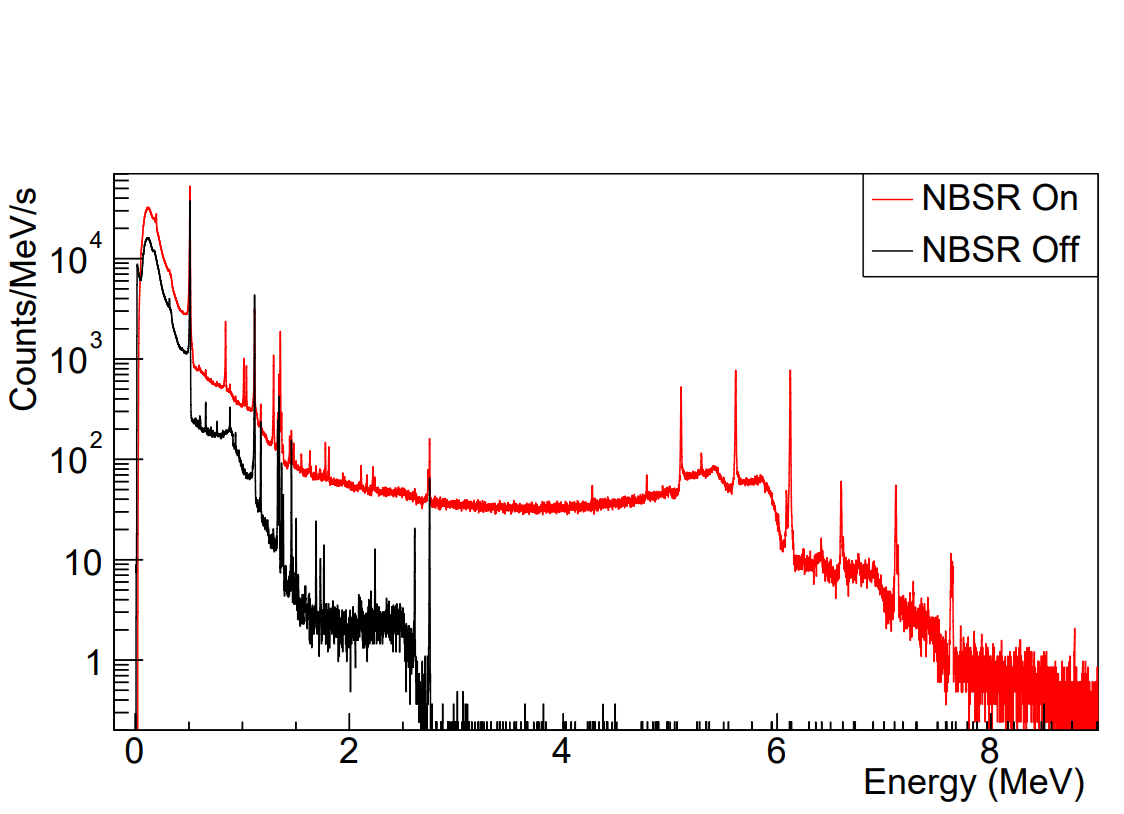
\includegraphics[width=0.7\linewidth]{Chapter2/Figs/Raster/Prospect_NSBR_gammaSpec.png}
 \captionof{figure}{Example HPGe $\gamma$-ray spectra taken with the NBSR on and off. Prominent lines, and associated escape peaks and Compton continua, are evident. From \cite{Ashenfelter_2016} (table 2 in \cite{Ashenfelter_2016} shows line sources).} 
 \label{fig:Prospect_NSBR_gammaSpec}
\end{figure}

\begin{figure}[!h]
 \centering
 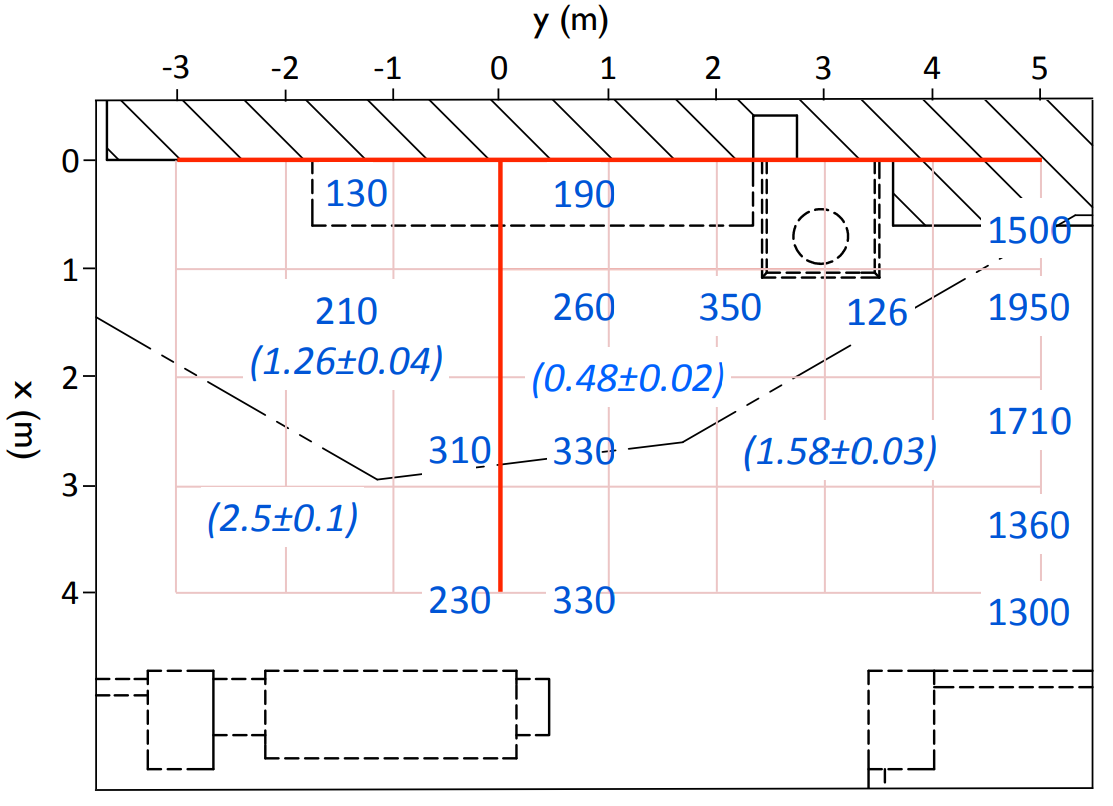
\includegraphics[width=0.7\linewidth]{Chapter2/Figs/Raster/prospectNeutronMap.png}
 \captionof{figure}{A pictorial representation of neutron dose rates (measured in nSv/h) and thermal neutron rates in italics (cm$^{-2}$ s${^-1}$) at the HFIR near location roughly 15\,cm (z = 0.15) above the floor. Measurements are plotted on a one meter square grid refernced to the ractor wall (x = 0) and the smallest baseline (y = 0). The reactor core is centred at (x,y,z) = (-4.06,0,-3.85). From \cite{Ashenfelter_2016} } 
 \label{fig:prospectNeutronMap}
\end{figure}

% \begin{figure}[!h]
%  \centering
%  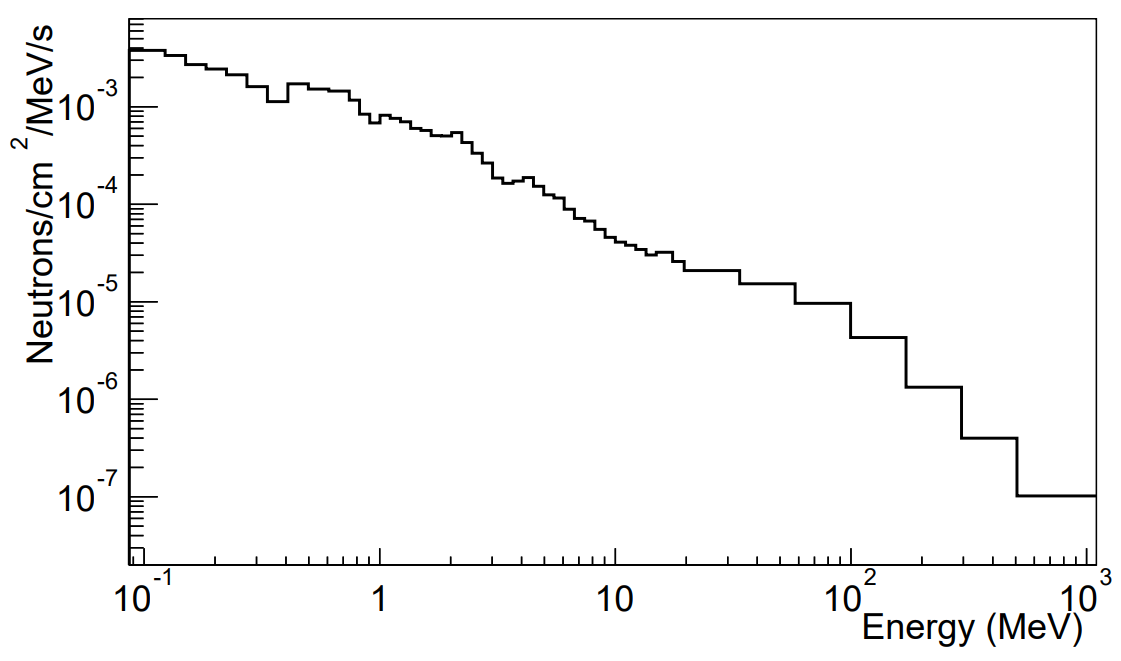
\includegraphics[width=0.7\linewidth]{Chapter2/Figs/Raster/JDEC_neutronSpec.png}
%  \captionof{figure}{The JEDEC standard fast neutron spectrum recorded at sea
% level in New York. From \cite{JEDEC_2006}. } 
%  \label{fig:JDEC_neutronSpec}
% \end{figure}

\begin{figure}[!h]
\centering
\begin{subfigure}{.5\textwidth}
  \centering
  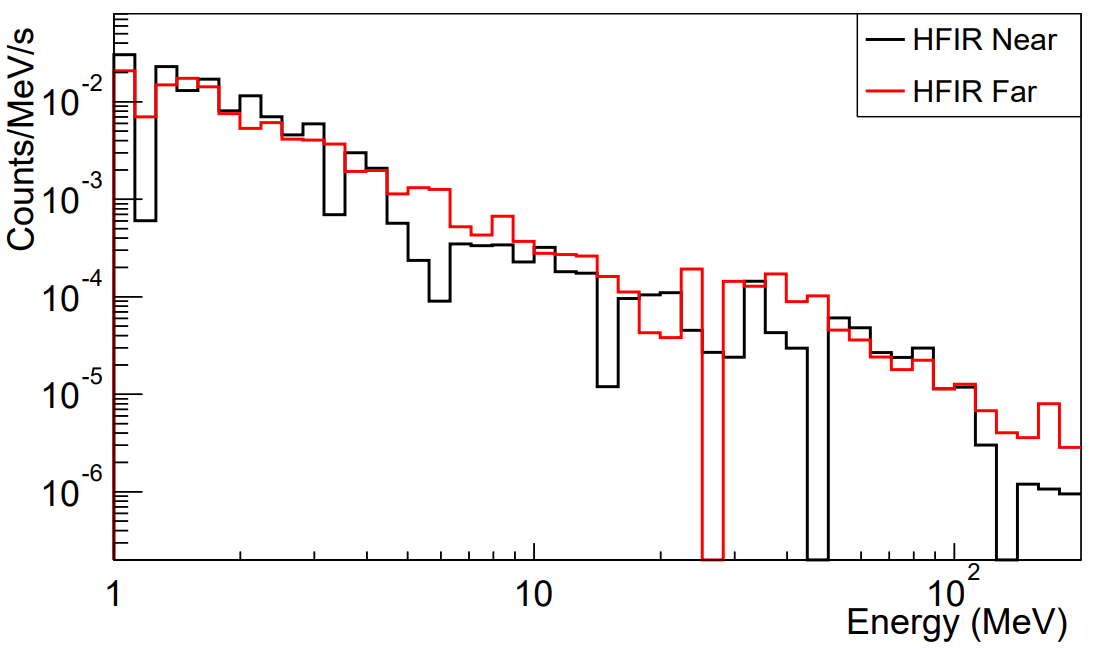
\includegraphics[width=\linewidth]{Chapter2/Figs/Raster/Prospect_HFIR_nearFarPlot.png}
  \captionsetup{width=.9\linewidth}
  \caption{}
  \label{subFig:Prospect_HFIR_nearFarPlot}
\end{subfigure}%
\begin{subfigure}{.5\textwidth}
  \centering
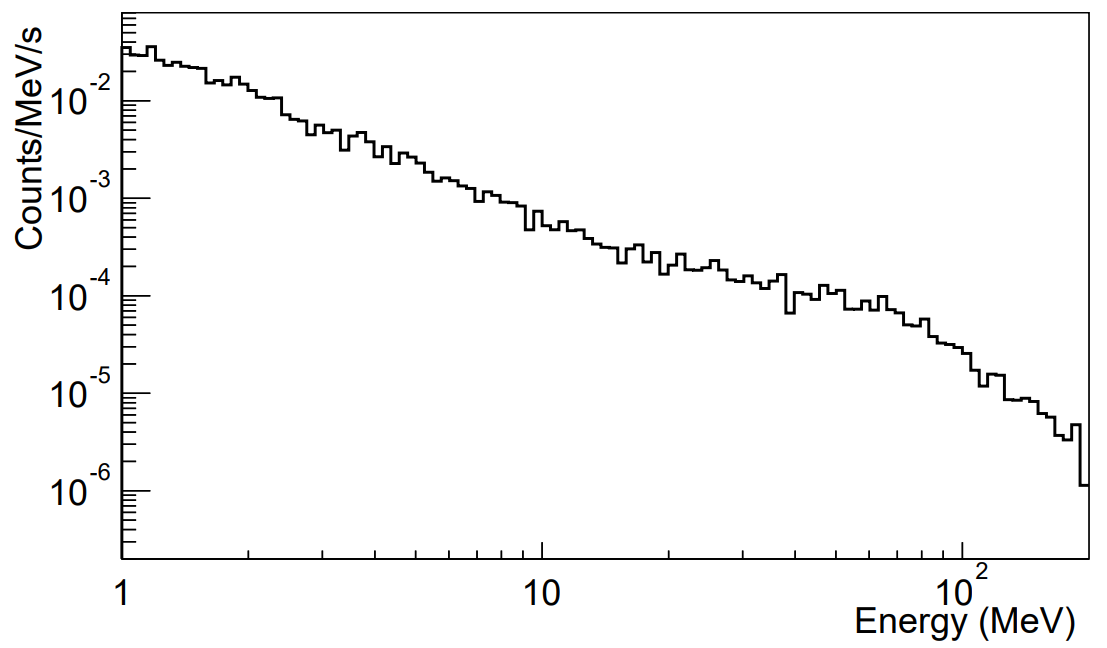
\includegraphics[width=\linewidth]{Chapter2/Figs/Raster/Prospect_NBSR_farPlot.png}
  \captionsetup{width=.9\linewidth}
  \caption{}
  \label{subFig:Prospect_NBSR_farPlot}
\end{subfigure}
\caption{The cosmogenic neutron-induced energy spectrum was recorded at the (a) HFIR near and far locations and (b) NBSR far location. From \cite{Ashenfelter_2016}.}
\label{fig:Prospect_HFIR_NBSR_nearFarPlots}
\end{figure}

\begin{figure}[!h]
 \centering
 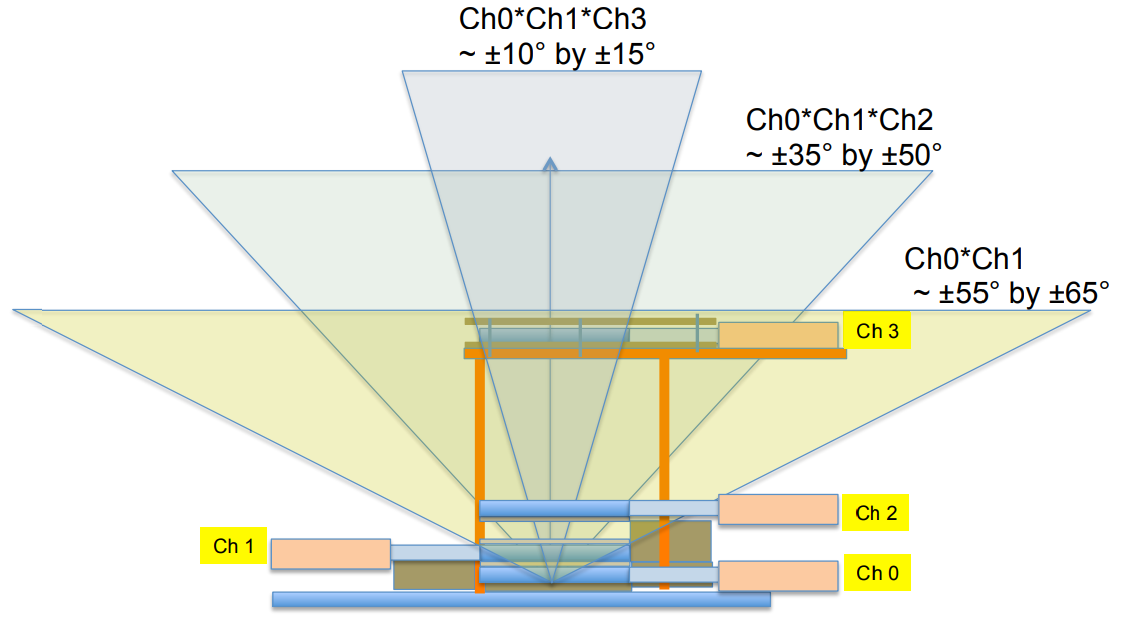
\includegraphics[width=0.7\linewidth]{Chapter2/Figs/Raster/Prospect_MuonPaddels.png}
 \captionof{figure}{The angular acceptances for the $\mu$ telescope instrument
used at all sites is determined by the coincidence requirement enforced
between the 4 plastic scintillator paddles. From \cite{Ashenfelter_2016}.} 
 \label{fig:Prospect_MuonPaddels}
\end{figure}

\section{The Upgraded Detector}\label{sec:theUpgradedDetector}
Please note that in the following section of text the term upgraded and VIDARR detector are used interchangeably. The upgraded detector will have 21 more layers than the prototype detector going from 49 to 70 layers. In addition, the 3 missing columns on side A are also now instrumented. This means the number of channels has increased from 1793 to 2660 which results in a mass increase of $\sim$ 50\,\%, thus improving the fiducial volume of the detector. This means that more energy from the gadolinium cascade is contained within the detector thus allowing for more effective noise reduction when triggering. Therefore the increase in layers will increase the amount of the 8\,MeV Gd cascade contained in the detector. The increase in layers will not yield a significant increase in e$^+$ efficiency as e$^+$s are effectively contained to a $\sim$ 99\,\% level with both 1793 channels and 2660 channels as they are contained within 1-2 bars.
\\\\The electronics have been improved significantly when compared to the original detector. The original electronics were carried over from the T2K Ecal. They were the first generation of this technology with relatively high noise rates compared to the current generation used in the VIDARR detector. The energy resolution of the electronics has been greatly increased. The noise rates for the original electronics were also more susceptible to changes in temperature than the electronics in the upgraded detector. In addition, the upgraded detector will also have field-programmable gate array (FPGA) boards that connect with analogue boards in turn connecting to the MPPCs. The use of FPGA boards will allow for more complex trigger functions to be used with up to two discriminating energy thresholds available. These discriminating energy thresholds will greatly improve the S/N ratio of triggering events. This will be achieved by looking at the summed energy and the number of bars hit past each threshold. As will be expanded upon later in section \ref{sec:MachineLearningTrigger} the improvement to energy resolution has a significant effect on the S/N ratio as well. During the analysis the lowest available threshold of $\sim$ 0.1\,MeV was the most effective in distinguishing signal from noise. This improvement is only possible due to the upgraded electronics. The use of two thresholds as opposed to one on the prototype also proved useful for improving generated neutron efficiency. 
%\\\\A basic cut investigation used a form of machine learning called a support vector machine (SVM) to determine the best cut and which dimensions gave the best separation. The cut was dominated by the number of bars hit at the lower threshold of 0.1\,MeV, the most accurate cut would have been utilising the number of bars hit above 0.1\,MeV and the summed energy above the 0.1\,MeV threshold. However due to the structure of the FPGA boards and their programming it was more prudent to use the number of bars hit above both the 0.1\,MeV thresholds and 0.5\,MeV threshold. The cost in classifier accuracy was minimal and it allowed for faster development of the FPGA firmware. 
\\\\To lessen temperature fluctuations in the VIDARR detector the cooling in and around the detector module has been greatly increased from the prototype. The original detector had six radiator fins on 2 sides of the detector which were primarily aimed at cooling the TFBs on each fin (see figure \ref{fig:detCon002_OldTearAway}). The upgraded VIDARR detector will also have these fins which will help cool the new boards but on the same 2 sides as the fins, there will also be two new radiators behind the fins which run the width and height of a side figure \ref{fig:detCon_RadiatorConstruction_RadiatorPiping} shows the radiators being constructed. The new active cooling the radiators will provide will remove large amounts of heat from the detector. This will allow for a more consistent temperature  thus reducing dark noise from the MPPCs below the original detector's levels. 

\section{Detector Construction}\label{sec:DetectorConstruction}
The detector construction was a process that was sadly disrupted due to the COVID-19 pandemic which is still ongoing. The detector construction originally started in November of 2018 with the cutting and painting of scintillation bars. These bars will increase mass by $\sim$ 50\,\%. This process was completed by December of 2018. Also in December of 2018, the original detector was moved out of the shipping container which housed it (figure \ref{fig:detCon000_TakeOut1}). It was then placed inside a cleanroom opened and disassembled (figure \ref{fig:detCon002_OldTearAway}). The original electronics were re-purposed from the T2K ECal. As a result, their timing resolution could be significantly improved upon. These improved electronics also increased the power draw and so an increase in active cooling is desired. Then new scintillator was purchased from Fermi-lab which was $\sim$ twice as long as required. This new scintillator was then cut (figure \ref{subFig:detCon003bb_CuttingScint}) so its dimensions match the old scintillating bars (152\,cm $\times$ 4\,cm $\times$ 1\,cm) and fit exactly inside the detector casing. Once this was done the edges of the freshly cut scintillator were arranged and painted with TiO$_2$ paint (figure \ref{subFig:detCon005b_PaintingEnds}) to help reflect the light. The cut and painted scintillator were then placed inside the housing for the detector  whilst it was in the cleanroom (figure \ref{fig:detCon006_RonInCleanRoom}).

\begin{figure}[!h]
\centering
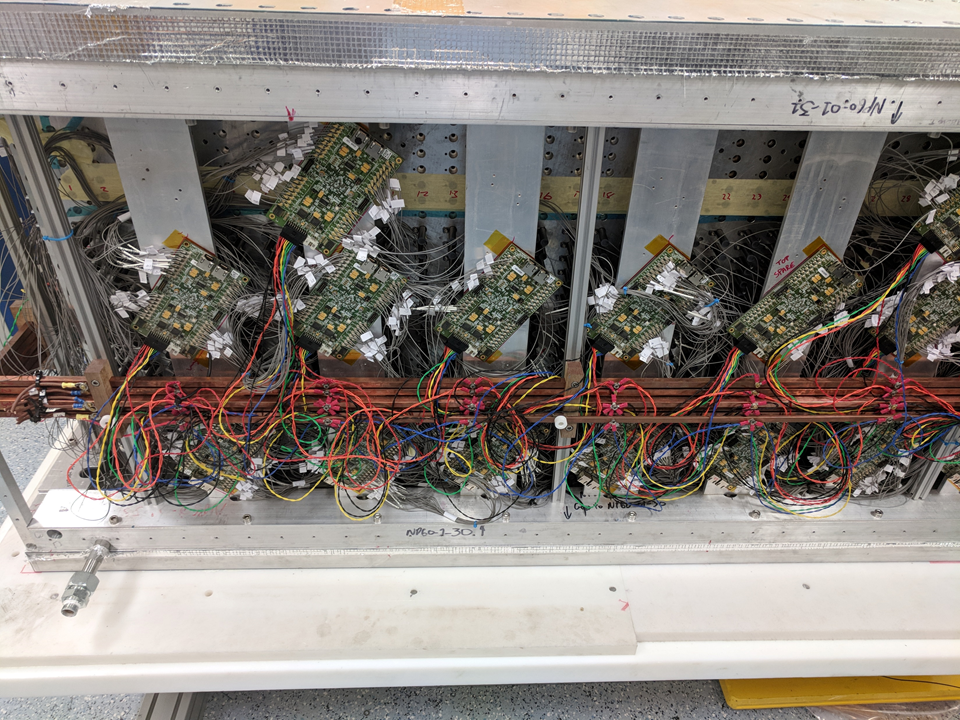
\includegraphics[width=0.8\linewidth]{Chapter3/Figs/Raster/detCon002_OldTearAway.png}
\captionof{figure}{A view of the electronics in the prototype detector. There is much available space between the boards and the detector itself. The cables are 100\,mm long.} 
\label{fig:detCon002_OldTearAway}
\end{figure}

\begin{figure}[!h]
\centering
\begin{subfigure}{.5\textwidth}
  \centering
  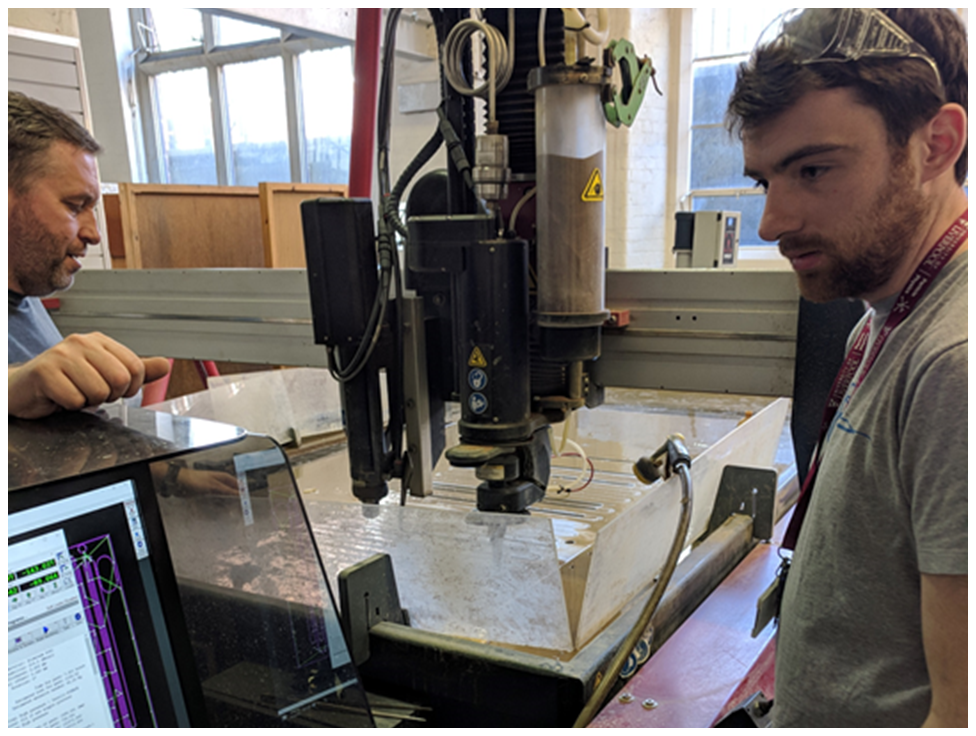
\includegraphics[width=\linewidth]{Chapter3/Figs/Raster/detCon011b_RadiatorConstruction.png}
  \captionsetup{width=.9\linewidth}
  \caption{The steel frame of the new radiator being cut .}
  \label{subFig:detCon011b_RadiatorConstruction}
\end{subfigure}%
\begin{subfigure}{.5\textwidth}
  \centering
  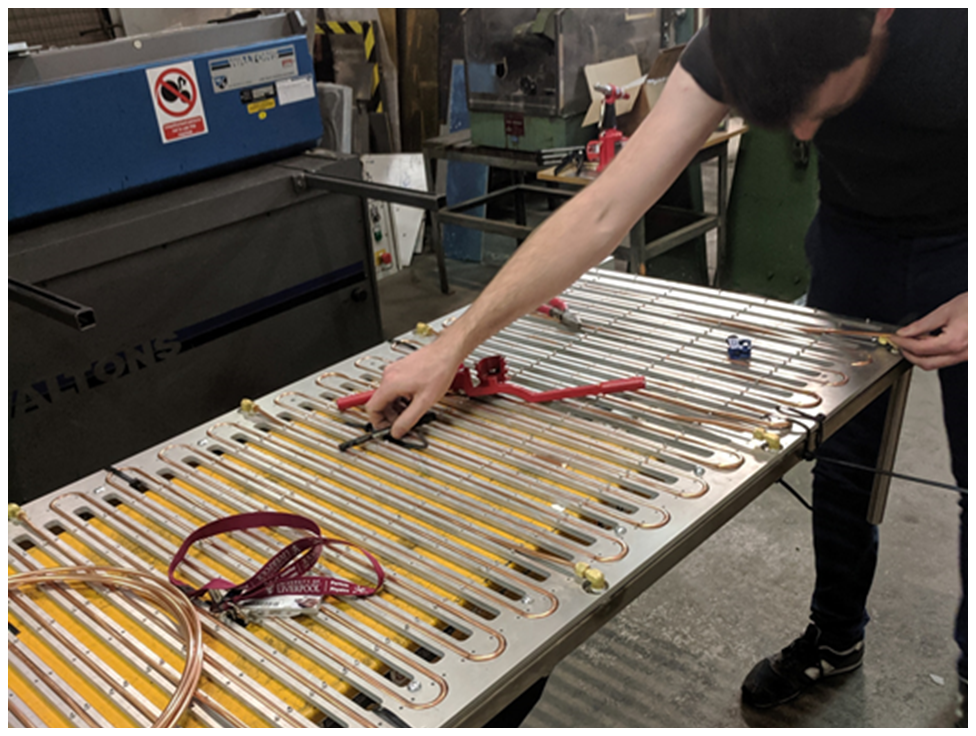
\includegraphics[width=\linewidth]{Chapter3/Figs/Raster/detCon012b_RadiatorPiping.png}
  \captionsetup{width=.9\linewidth}
  \caption{The new radiator having the piping inserted.}
  \label{subFig:detCon012b_RadiatorPiping}
\end{subfigure}
\caption{The construction of the new radiator has more active cooling and a larger surface area than the original radiator. \hl{numbers for cooling anywhere?}}
\label{fig:detCon_RadiatorConstruction_RadiatorPiping}
\end{figure}

\begin{figure}[!h]
\centering
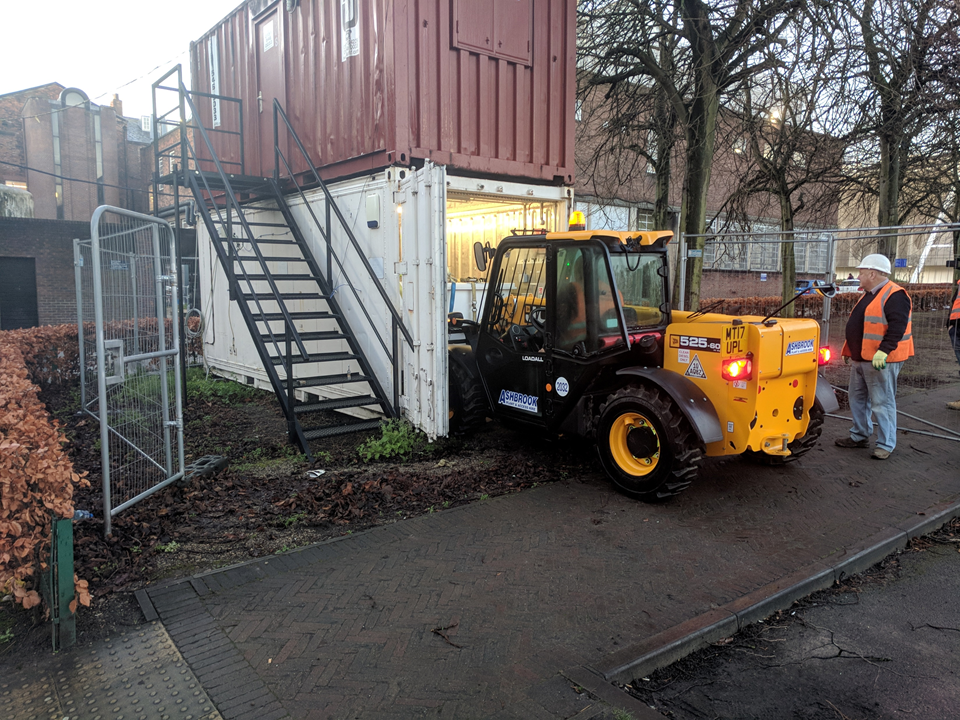
\includegraphics[width=0.8\linewidth]{Chapter3/Figs/Raster/detCon000_TakeOut1.png}
\captionof{figure}{The prototype detector being taken out of the original shipping container which was a standard cool ``meat locker.''} 
\label{fig:detCon000_TakeOut1}
\end{figure}

\begin{figure}[!h]
\centering
\begin{subfigure}{.5\textwidth}
  \centering
  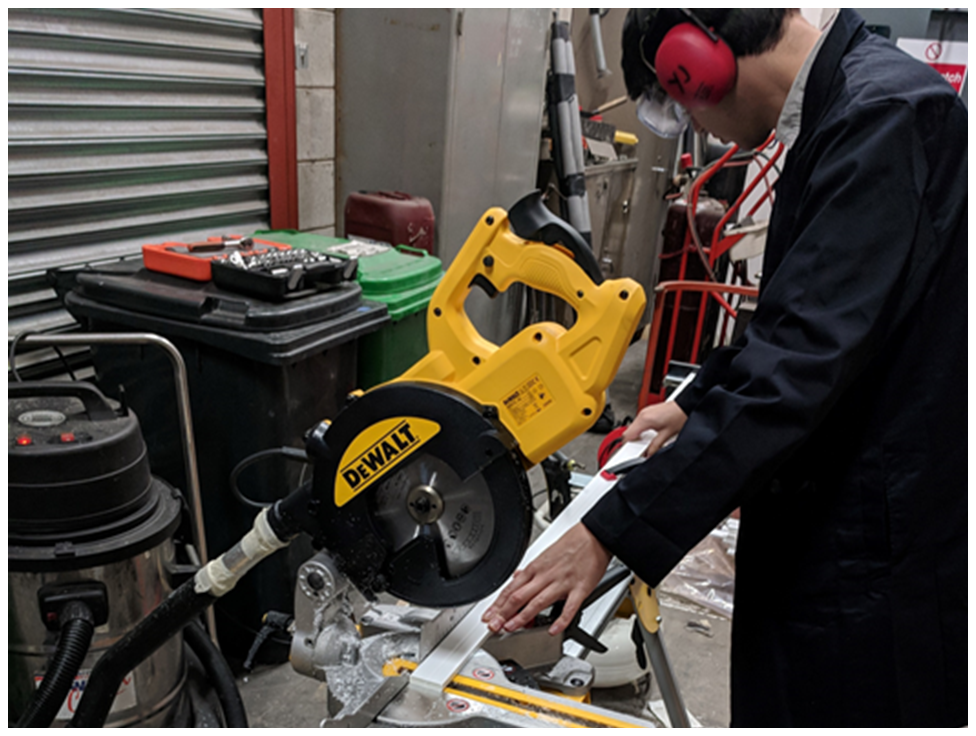
\includegraphics[width=\linewidth]{Chapter3/Figs/Raster/detCon003bb_CuttingScint.png}
  \captionsetup{width=.9\linewidth}
  \caption{Fellow collaborator Yan-Jie Schnellbach cutting scintillator.}
  \label{subFig:detCon003bb_CuttingScint}
\end{subfigure}%
\begin{subfigure}{.5\textwidth}
  \centering
  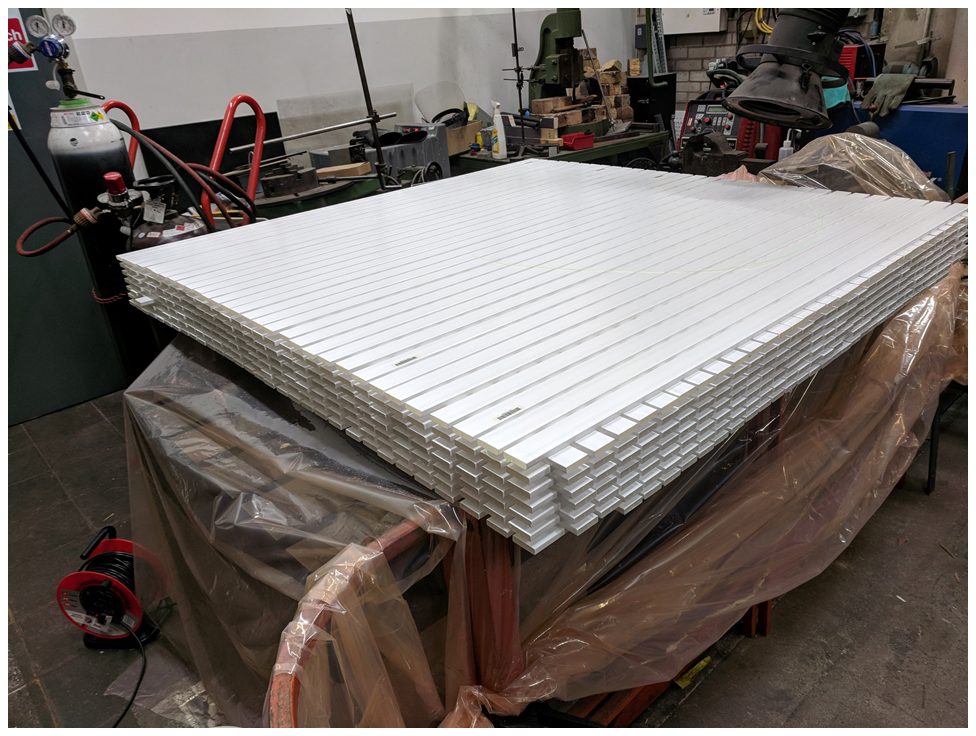
\includegraphics[width=\linewidth]{Chapter3/Figs/Raster/detCon005b_PaintingEnds.png}
  \captionsetup{width=.9\linewidth}
  \caption{The scintillator being arranged for painting the ends of the scintillator.}
  \label{subFig:detCon005b_PaintingEnds}
\end{subfigure}
\caption{Scintillator preparation for being placed inside the detector casing.}
\label{fig:detCon_CuttingScint_PaintingEnds}
\end{figure}

\begin{figure}[!h]
\centering
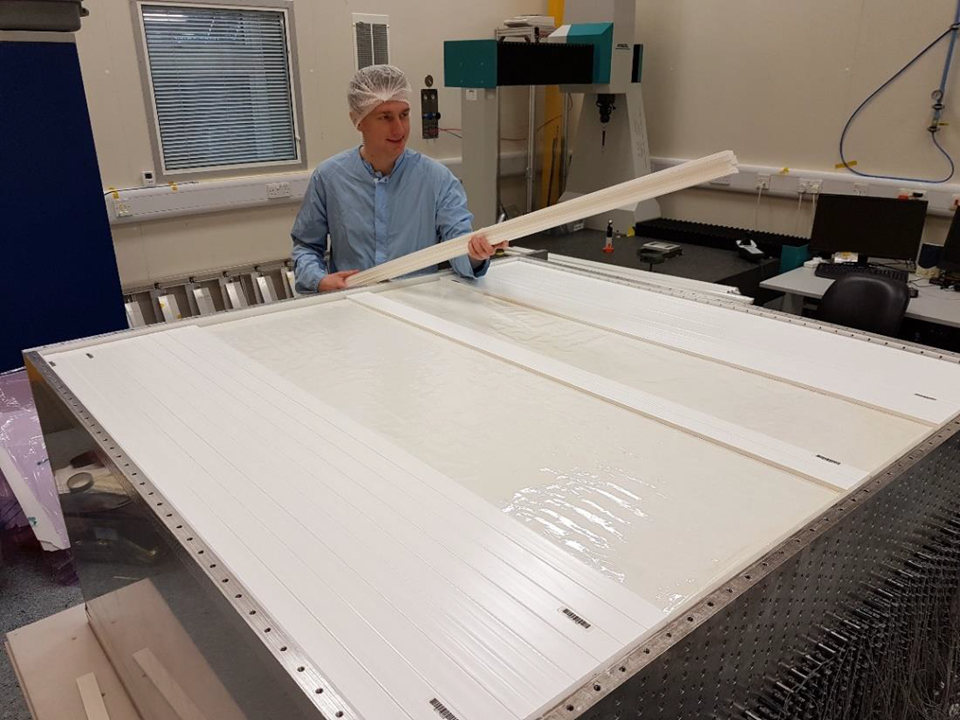
\includegraphics[width=0.8\linewidth]{Chapter3/Figs/Raster/detCon006_RonInCleanRoom.png}
\captionof{figure}{Me (Ronald Collins) in the cleanroom putting scintillator into the detector. The white sheet of Gadolinium Oxide in-between the layers is also visible.} 
\label{fig:detCon006_RonInCleanRoom}
\end{figure}

One of the major improvements made during the upgrade of the VIDARR detector was an increase in cooling. The original detector had much space between the electronic boards and the MPPCs with the electronic boards placed directly on cooling fins (see in figure \ref{fig:detCon002_OldTearAway}). In addition to the cooling fins seen in figure \ref{fig:detCon002_OldTearAway} large radiators have now been added in-between the cooling fins and the MPPCs for each side. These new radiators are comprised of large stainless steel plates which were cut using a water cutter shown in figure \ref{subFig:detCon011b_RadiatorConstruction}. Then copper piping was placed through the sections seen in figure \ref{subFig:detCon012b_RadiatorPiping}. This copper piping will face the MPPCs and the detector scintillator whilst the radiator fins will be attached behind the radiator away from the MPPCs and behind the insulation. As in the prototype, the electronic boards will be placed on the fins similar to figure \ref{fig:detCon002_OldTearAway}. This should improve the cooling in the detector significantly as the heat from the electronic boards should be isolated from the scintillator and the MPPCs when compared to the prototype. 

Once the scintillator is in the detector casing several individual components need to be assembled so that the light emitted by the scintillator can then be analysed. A small amount of light emitted by the scintillator upon particle interaction is trapped by the WLS fibres . These fibres are threaded through the centre of the scintillator and capture light and shift it to green light seen in figure \ref{subFig:detCon013b_WlsFibres}. These WLS fibres then have 3d printed connectors glued to the ends of them as seen in figure \ref{subFig:detCon014b_WlsWithEnds}. Then the MPPC's connectors are 3D printed seen both with the support struts in figure \ref{subFig:detCon015b_3dPrintedHolders} and without in figure \ref{subFig:detCon016b_3dPrintedFreed}. Then the holders for the MPPCs which attach to the Then PCBs which connect the MPPCs to the coaxial cables need to be produced. A sheet of which can be seen in figure \ref{subFig:detCon008b_PlacingPcbs}. These PCBs have to have a coaxial cable connector soldered on to them and pins pushed through them so they can pick up the signals that the MPPCs produce. A finished example of one of these PCBs can be seen in figure \ref{subFig:detCon009b_SoloPcb}. The holders PCBs and MPPCs all fit together as shown in figure \ref{fig:detCon017b_HoldersWithParts}.

\begin{figure}[!h]
\centering
\begin{subfigure}{.5\textwidth}
  \centering
  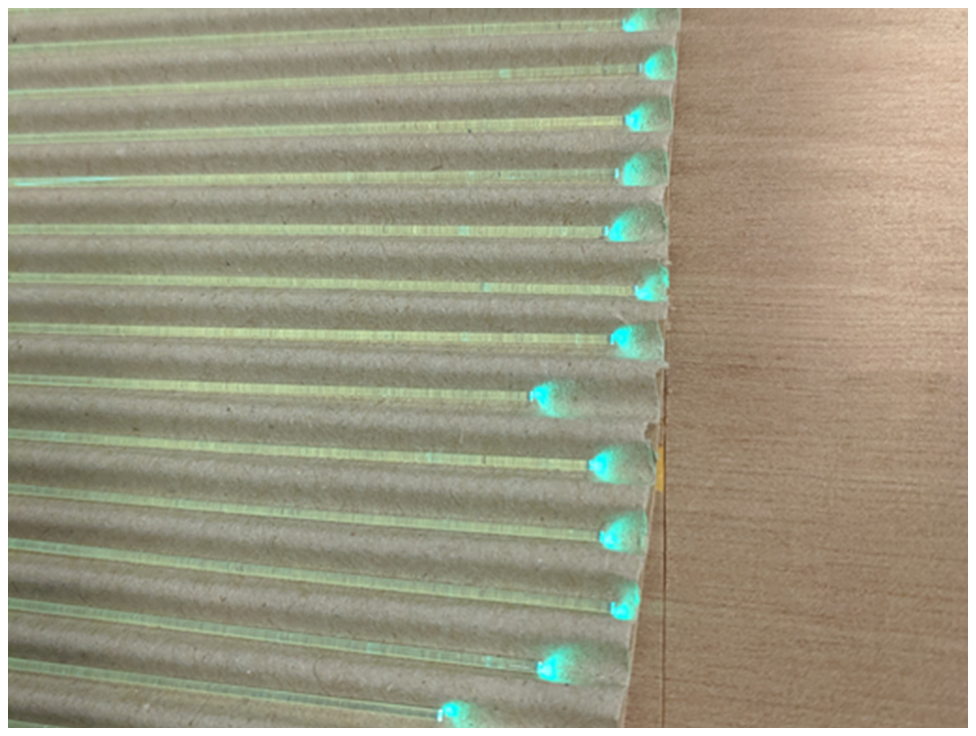
\includegraphics[width=\linewidth]{Chapter3/Figs/Raster/detCon013b_WlsFibres.png}
  \captionsetup{width=.9\linewidth}
  \caption{The WLS fibres are threaded into the scintillator.}
  \label{subFig:detCon013b_WlsFibres}
\end{subfigure}%
\begin{subfigure}{.5\textwidth}
  \centering
  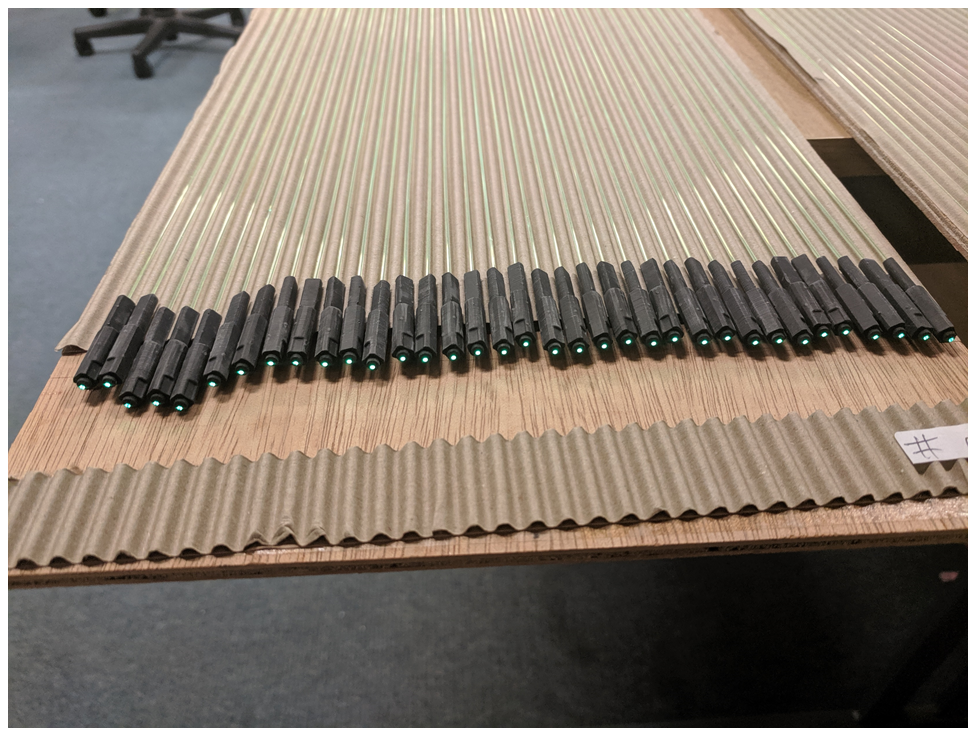
\includegraphics[width=\linewidth]{Chapter3/Figs/Raster/detCon014b_WlsWithEnds.png}
  \captionsetup{width=.9\linewidth}
  \caption{The WLS fibres with ends that connect to the plastic holders which house the MPPCs.}
  \label{subFig:detCon014b_WlsWithEnds}
\end{subfigure}
\caption{The WLS fibres will funnel light from the scintillator to the MPPCs. They are assembled on cardboard and have 3d printed ends glued onto them.}
\label{fig:detCon_WlsFibres_WlsWithEnds}
\end{figure}

\begin{figure}[!h]
\centering
\begin{subfigure}{.5\textwidth}
  \centering
  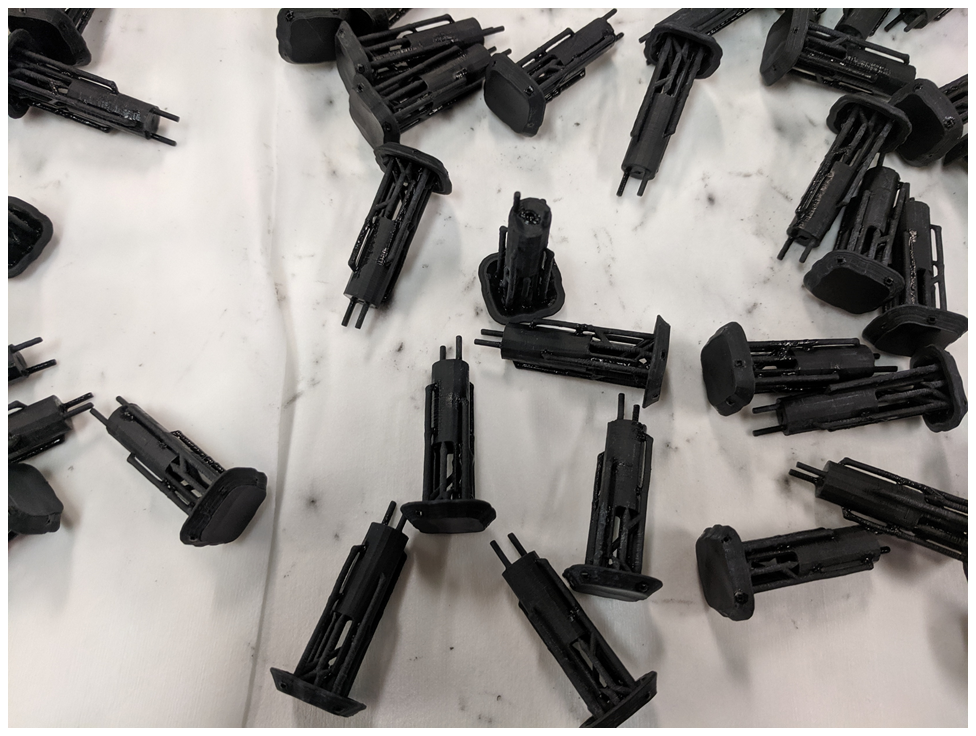
\includegraphics[width=\linewidth]{Chapter3/Figs/Raster/detCon015b_3dPrintedHolders.png}
  \captionsetup{width=.9\linewidth}
  \caption{3D printed holders for the MPPCs and PCBs with supporting struts.}
  \label{subFig:detCon015b_3dPrintedHolders}
\end{subfigure}%
\begin{subfigure}{.5\textwidth}
  \centering
  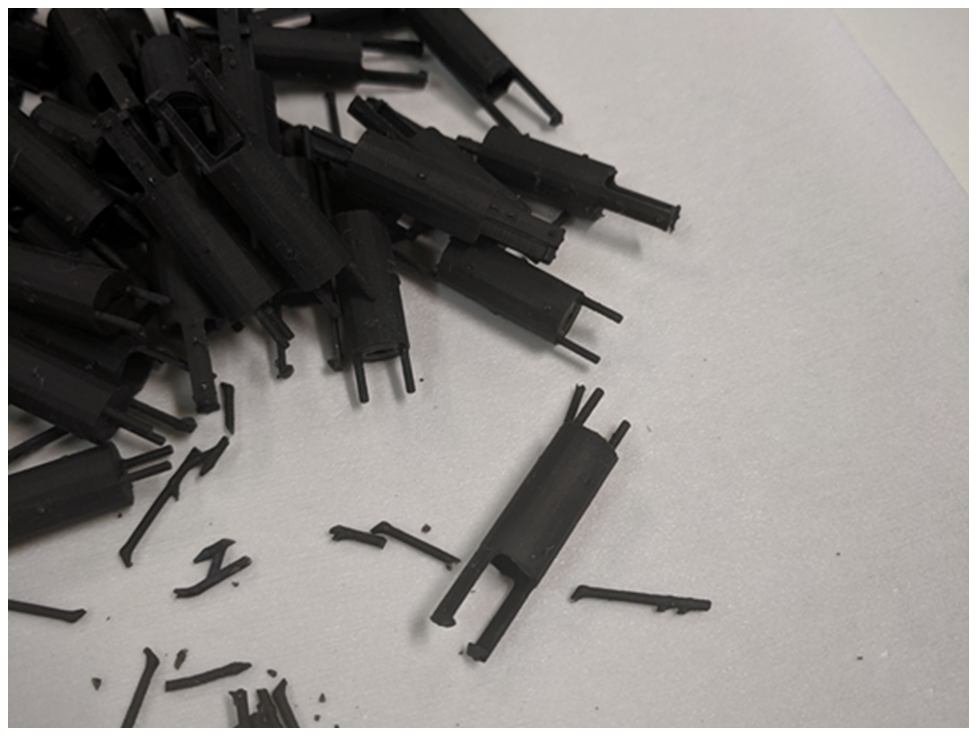
\includegraphics[width=\linewidth]{Chapter3/Figs/Raster/detCon016b_3dPrintedFreed.png}
  \captionsetup{width=.9\linewidth}
  \caption{3D printed holders for the MPPCs and PCBs freed from their struts .}
  \label{subFig:detCon016b_3dPrintedFreed}
\end{subfigure}
\caption{The holders for the MPPCs and the PCBs. Holders for the additional channels needed to be 3D printed as more from the original supply chain could not be procured. }
\label{fig:detCon_3dPrintedHolders_3dPrintedFreed}
\end{figure}

\begin{figure}[!h]
\centering
\begin{subfigure}{.5\textwidth}
  \centering
  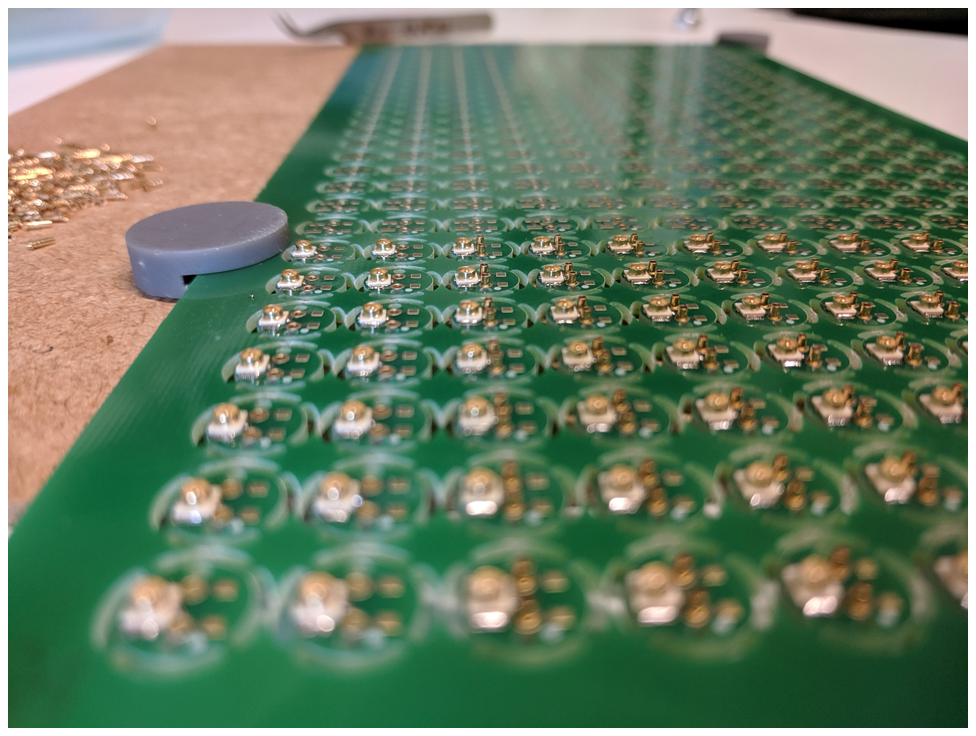
\includegraphics[width=\linewidth]{Chapter3/Figs/Raster/detCon008b_PlacingPcbs.png}
  \captionsetup{width=.9\linewidth}
  \caption{A sheet of PCB boards being assembled. Slightly elevated for putting in  pins.}
  \label{subFig:detCon008b_PlacingPcbs}
\end{subfigure}%
\begin{subfigure}{.5\textwidth}
  \centering
  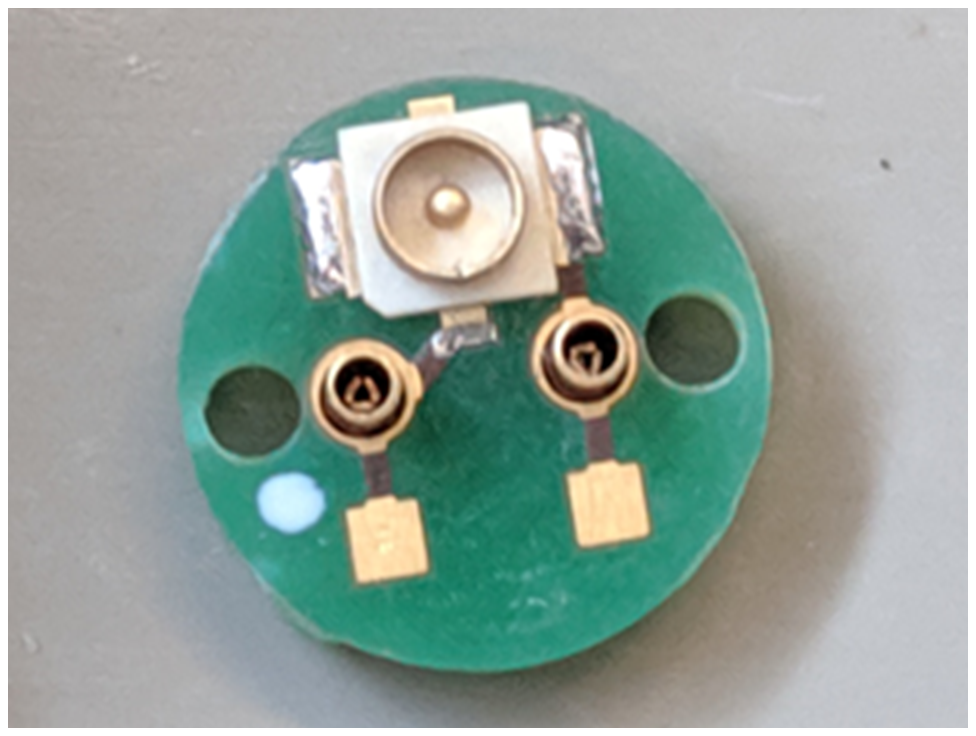
\includegraphics[width=\linewidth]{Chapter3/Figs/Raster/detCon009b_SoloPcb.png}
  \captionsetup{width=.9\linewidth}
  \caption{A finished solo PCB that connects to the MPPC.}
  \label{subFig:detCon009b_SoloPcb}
\end{subfigure}
\caption{The assembly of the PCBs which attach to the MPPCs through pins. The connector at the top of the PCBs is where the cables are attached.}
\label{fig:detCon_PlacingPcbs_SoloPcb}
\end{figure}

\begin{figure}[!h]
\centering
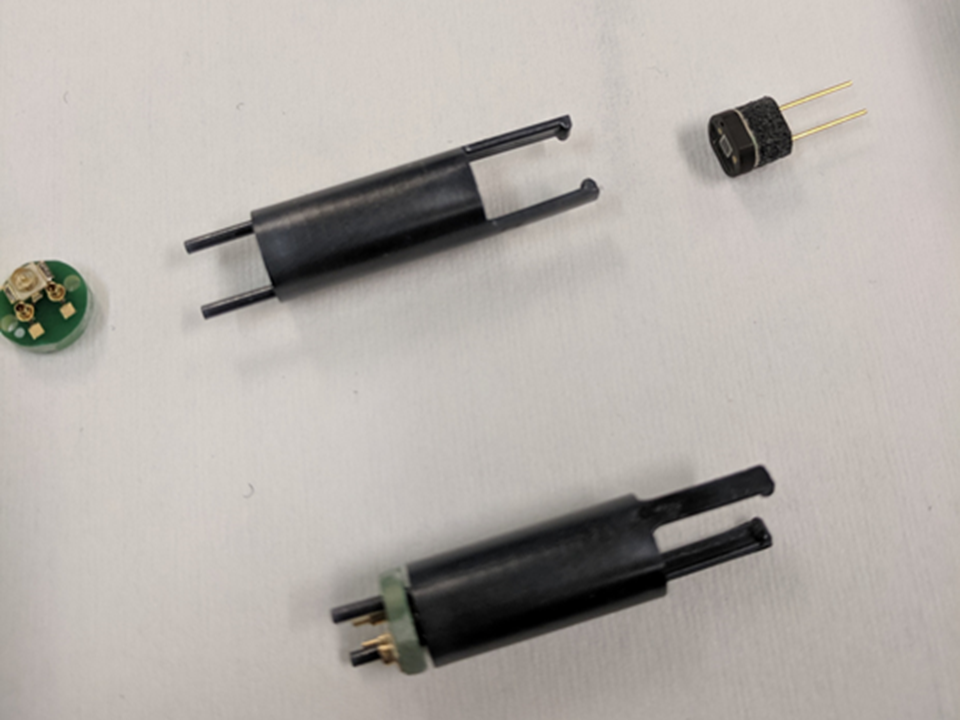
\includegraphics[width=0.8\linewidth]{Chapter3/Figs/Raster/detCon017b_HoldersWithParts.png}
\captionof{figure}{Holder next to MPPC and PCB (Top) and holder with assembled components (Bottom). Note the MPPC in the top right is actually reversed from its correct orientation, the prongs of the MPPC go through the PCB board pins.} 
\label{fig:detCon017b_HoldersWithParts}
\end{figure}

The next step was to label the coaxial cables. These cables connect the PCBs in figure \ref{fig:detCon_PlacingPcbs_SoloPcb} to the analogue boards. The labels are printed out by the machine seen in figure  \ref{subFig:detCon018b_HeatLabelsPrinted}. This machine prints the labels in long streams which then need to be cut into individual labels seen in figure \ref{subFig:detCon019b_CutLabels}. The label syntax is side-row-column with the bottom left of each side being the coordinate for (0,0). These labels are then slid onto the coaxial cables 8\,cm from the end that connects to the analogue boards as seen in figure \ref{subFig:detCon020b_LabelsLoose}. A heat gun is used to shrink the labels onto the coaxial cables as seen in figure \ref{subFig:detCon021b_LabelsHeated}. These cables are then connected to the holders where the PCB connector seen in figure \ref{subFig:detCon009b_SoloPcb} connects firmly to the cable. The holder is also put into a sheath so that it is held firmly in place once inside the detector, as seen in figure \ref{fig:detCon023b_HoldersConnectedZoom}.

\begin{figure}[!h]
\centering
\begin{subfigure}{.5\textwidth}
  \centering
  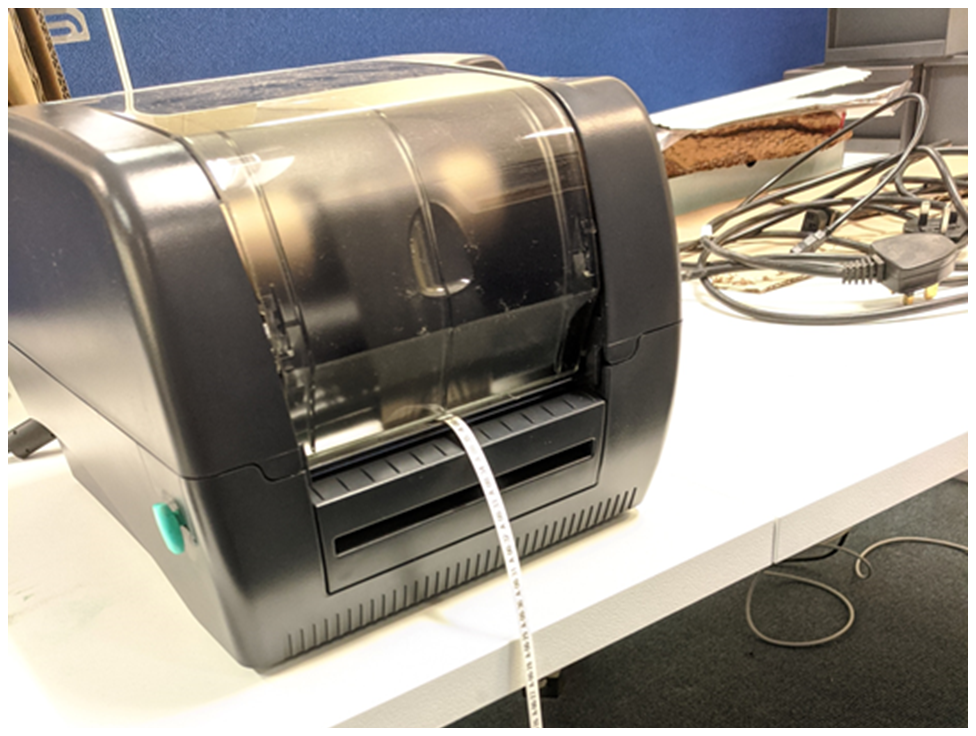
\includegraphics[width=\linewidth]{Chapter3/Figs/Raster/detCon018b_HeatLabelsPrinted.png}
  \captionsetup{width=.9\linewidth}
  \caption{Heat shrink labels being printed out.}
  \label{subFig:detCon018b_HeatLabelsPrinted}
\end{subfigure}%
\begin{subfigure}{.5\textwidth}
  \centering
  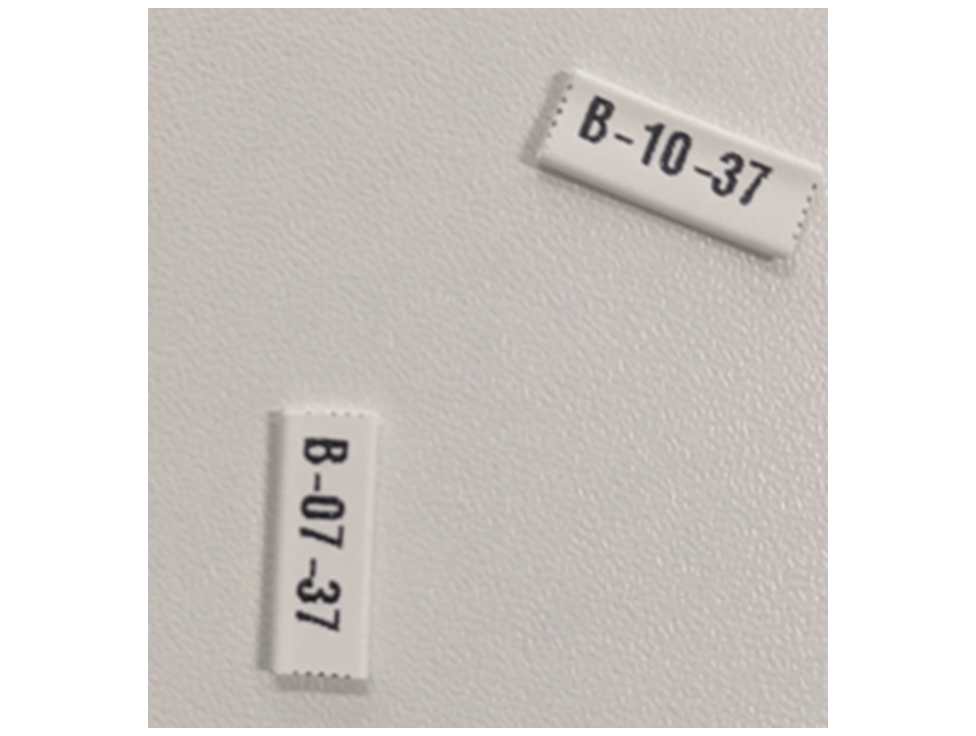
\includegraphics[width=\linewidth]{Chapter3/Figs/Raster/detCon019b_CutLabels.png}
  \captionsetup{width=.9\linewidth}
  \caption{Individual labels for specific cables.}
  \label{subFig:detCon019b_CutLabels}
\end{subfigure}
\caption{Heat-shrink labels are used to identify cables. Labels are printed out in the form side-Row-Column where the bottom left is (0,0) }
\label{fig:detCon_HeatLabelsPrinted_CutLabels}
\end{figure}

\begin{figure}[!h]
\centering
\begin{subfigure}{.5\textwidth}
  \centering
  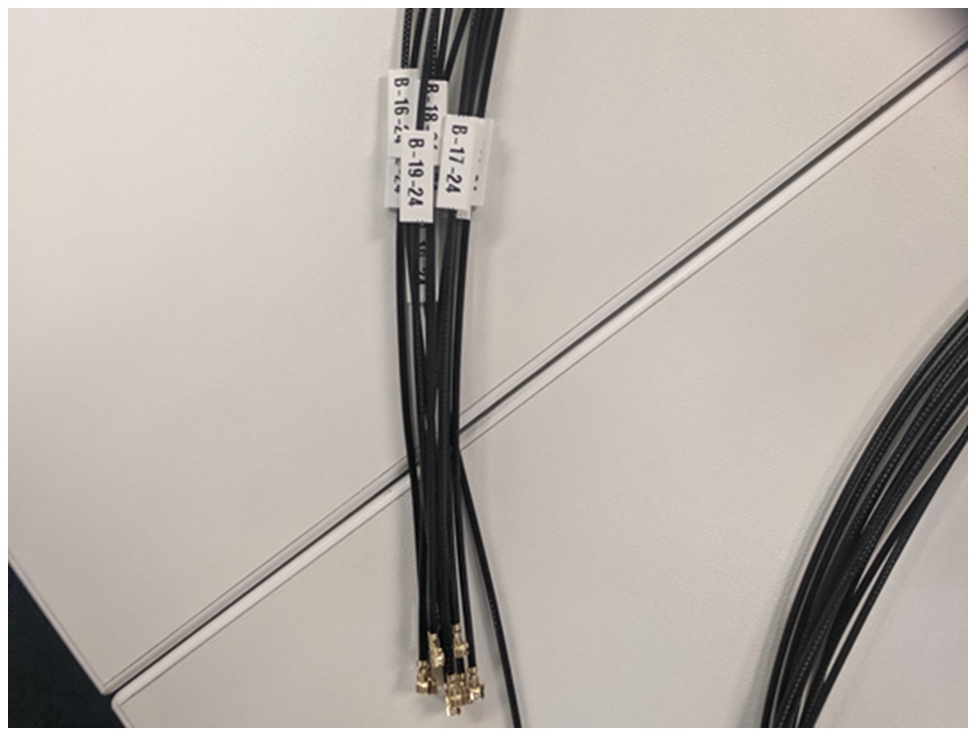
\includegraphics[width=\linewidth]{Chapter3/Figs/Raster/detCon020b_LabelsLoose.png}
  \captionsetup{width=.9\linewidth}
  \caption{Labels threaded onto the cables loosely .}
  \label{subFig:detCon020b_LabelsLoose}
\end{subfigure}%
\begin{subfigure}{.5\textwidth}
  \centering
  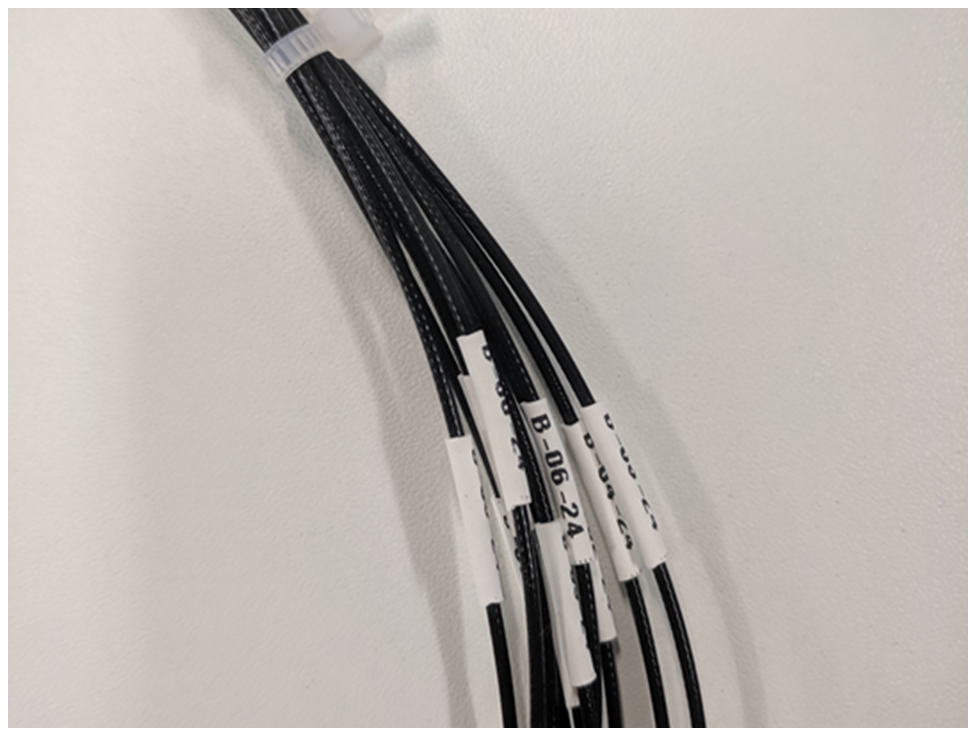
\includegraphics[width=\linewidth]{Chapter3/Figs/Raster/detCon021b_LabelsHeated.png}
  \captionsetup{width=.9\linewidth}
  \caption{The heated labels have shrunk.}
  \label{subFig:detCon021b_LabelsHeated}
\end{subfigure}
\caption{Labels are threaded through at 8\,cm from the end of the cables as seen in \ref{subFig:detCon020b_LabelsLoose} then a heat gun is used on the cables to shrink the labels and they are bunched as seen in in \ref{subFig:detCon021b_LabelsHeated}.}
\label{fig:detCon_LabelsLoose_LabelsHeated}
\end{figure}

\begin{figure}[!h]
\centering
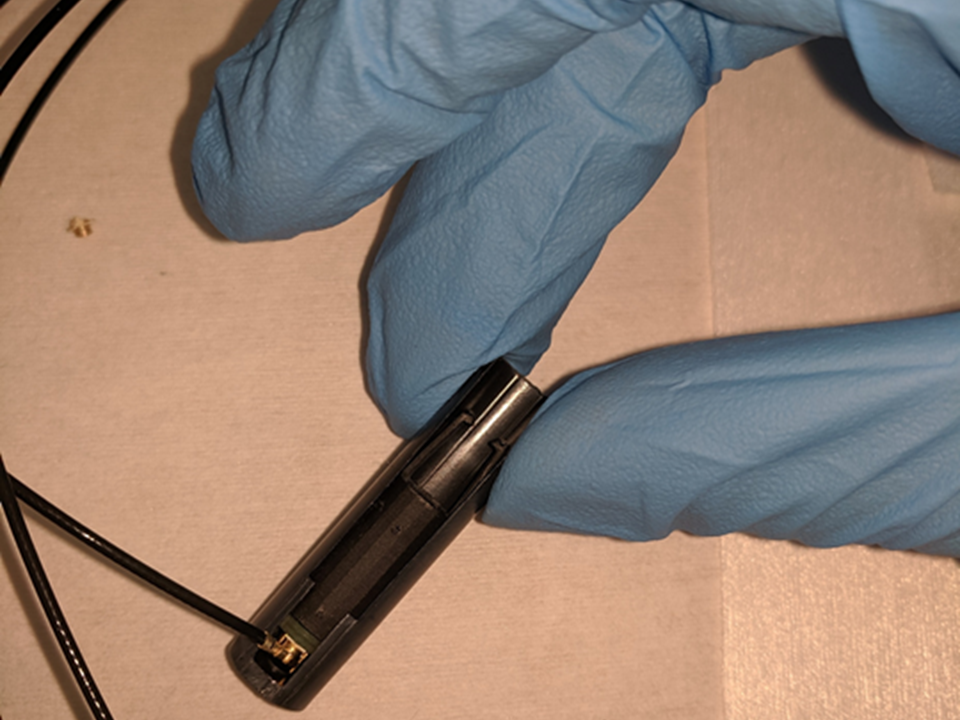
\includegraphics[width=0.8\linewidth]{Chapter3/Figs/Raster/detCon023b_HoldersConnectedZoom.png}
\captionof{figure}{The holder is connected to a cable and put inside a sheath.} 
\label{fig:detCon023b_HoldersConnectedZoom}
\end{figure}

All of the MPPC holders in their sheaths with connected cables are then attached to the WLS fibres and their 3D printed connectors shown in figure \ref{subFig:detCon014b_WlsWithEnds}. There are two distinct sheath types: grey made via injection moulding and orange sheaths which were 3d printed. These sheaths protect the rest of the components and can be seen clearly in figure \ref{fig:detCon_HaningOffRadiator_RadiatorTopDown} as they protrude from the detector casing. The radiator was slowly moved into position as cables were threaded through the insulation as can be seen in figure \ref{subFig:detCon026b_HaningOffRadiator}. Once the radiator was moved into position the space between the radiator and sheaths was checked to ensure that no undue pressure was being applied to the sheaths, which as figure \ref{subFig:detCon028b_RadiatorTopDown} shows there wasn't. Once the radiator was in position the cooling fins were also attached as seen in figure \ref{fig:detCon030b_RadiatorWithFins}. Also in figure \ref{fig:detCon030b_RadiatorWithFins} the x shaped analogue board holders have been attached via thermal paste to the cooling fins. An example of how the analogue boards are attached to the cooling fins can be seen in figure \ref{fig:detCon032_ConnectedBoard}. Which shows how the cables are connected to the analogue boards and aligned through an orange cable comb. 

\begin{figure}[!h]
\centering
\begin{subfigure}{.5\textwidth}
  \centering
  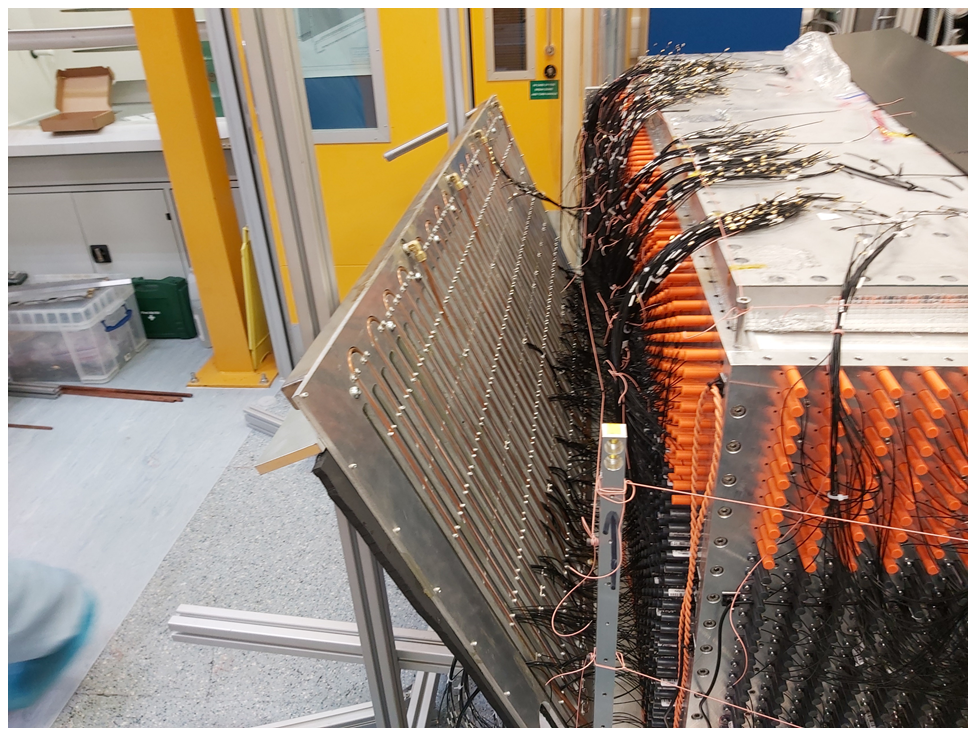
\includegraphics[width=\linewidth]{Chapter3/Figs/Raster/detCon026b_HaningOffRadiator.png}
  \captionsetup{width=.9\linewidth}
  \caption{The side A radiator being positioned into place as cables are placed through the insulation on the radiator.}
  \label{subFig:detCon026b_HaningOffRadiator}
\end{subfigure}%
\begin{subfigure}{.5\textwidth}
  \centering
  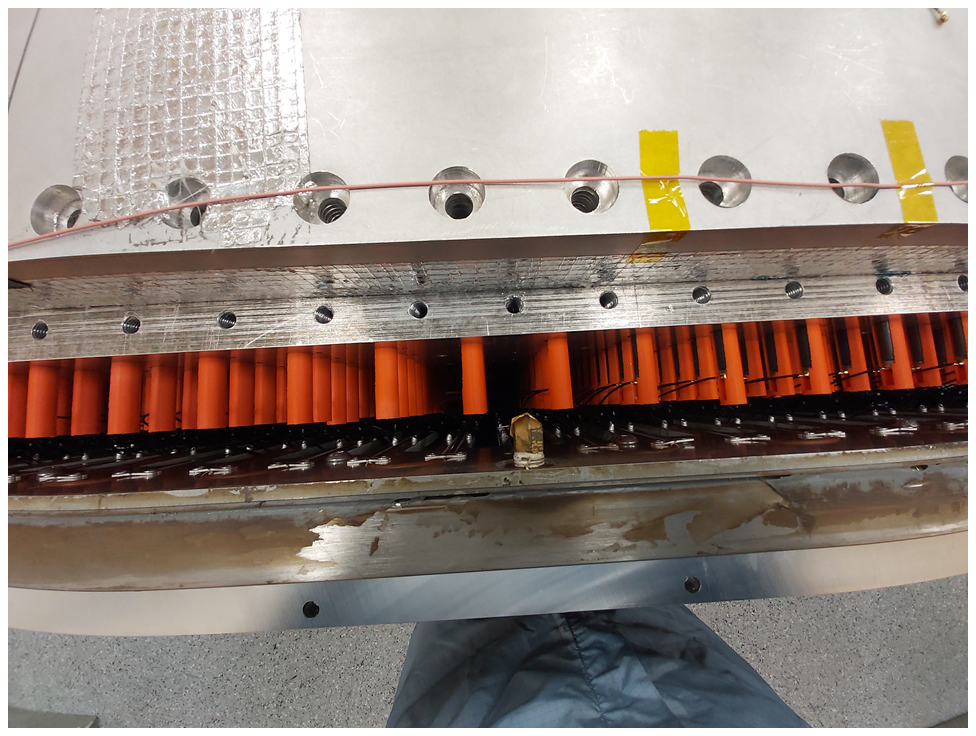
\includegraphics[width=\linewidth]{Chapter3/Figs/Raster/detCon028b_RadiatorTopDown.png}
  \captionsetup{width=.9\linewidth}
  \caption{The side A radiator is in position with all of the cables threaded through the insulation. There is minimal space.}
  \label{subFig:detCon028b_RadiatorTopDown}
\end{subfigure}
\caption{As part of the upgrade, the radiators are significantly larger and do not leave much space between the detector and the electronics.}
\label{fig:detCon_HaningOffRadiator_RadiatorTopDown}
\end{figure}

% \begin{figure}[!h]
% \centering
% \begin{subfigure}{.5\textwidth}
%   \centering
%   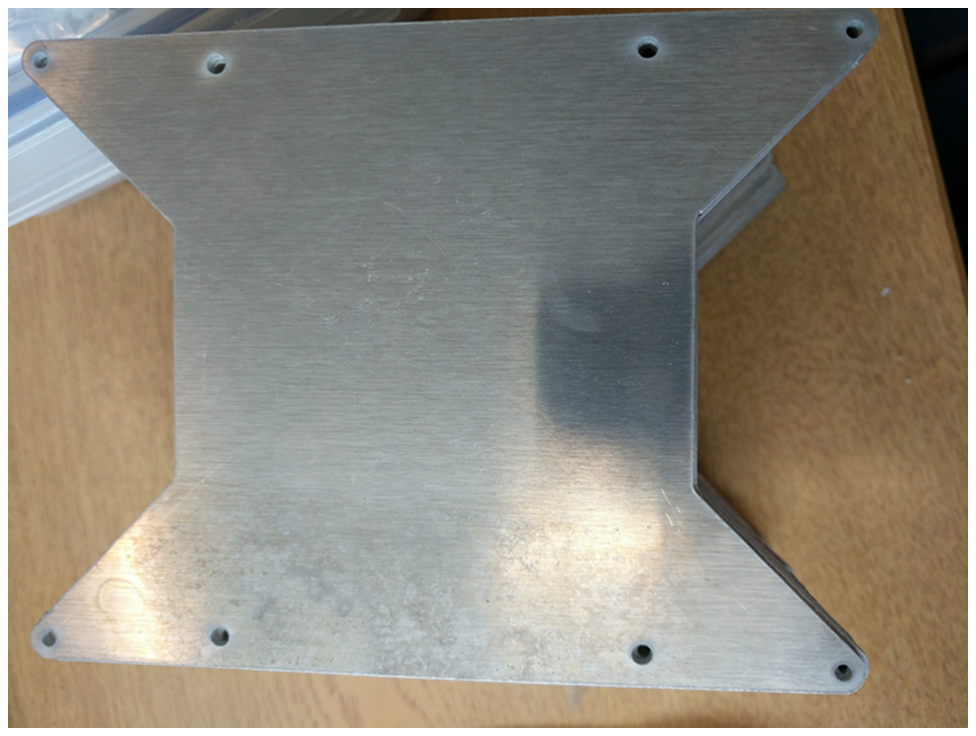
\includegraphics[width=\linewidth]{Chapter3/Figs/Raster/detCon029b_coolantFin.png}
%   \captionsetup{width=.9\linewidth}
%   \caption{Board holders that connect the analogue boards to the cooling fins.}
%   \label{subFig:detCon029b_coolantFin}
% \end{subfigure}%
% \begin{subfigure}{.5\textwidth}
%   \centering
%   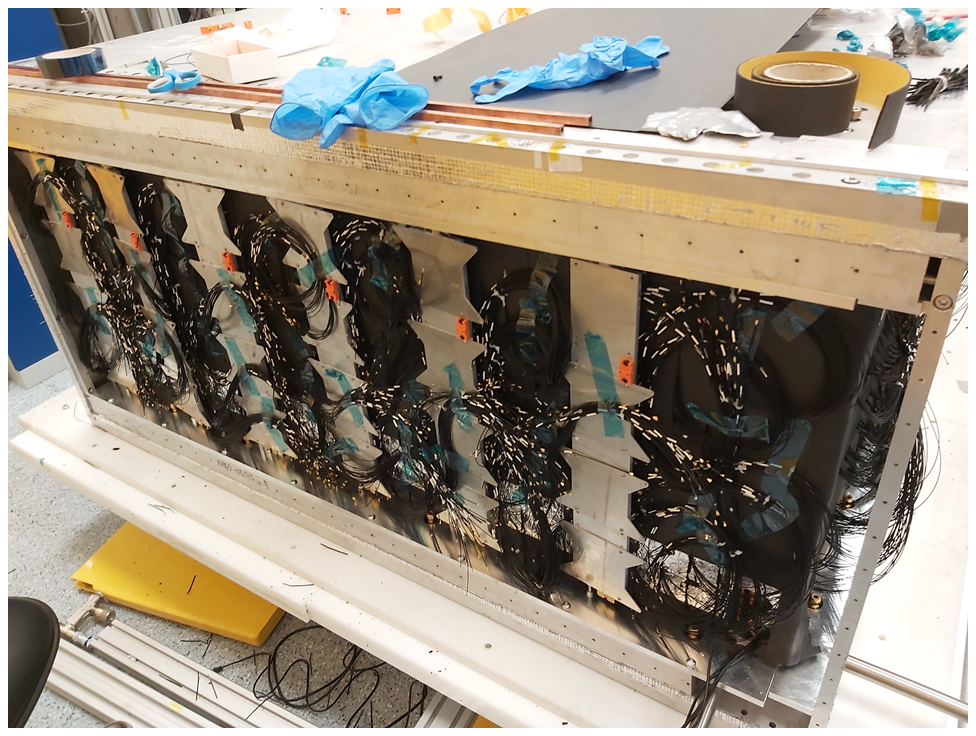
\includegraphics[width=\linewidth]{Chapter3/Figs/Raster/detCon030b_RadiatorWithFins.png}
%   \captionsetup{width=.9\linewidth}
%   \caption{Cooling fins and board holders attached to the radiator.}
%   \label{subFig:detCon030b_RadiatorWithFins}
% \end{subfigure}
% \caption{The analogue board holders and cooling fins are attached after the cables are threaded through the radiator insulation.}
% \label{fig:detCon_coolantFin_RadiatorWithFins}
% \end{figure}

\begin{figure}[!h]
\centering
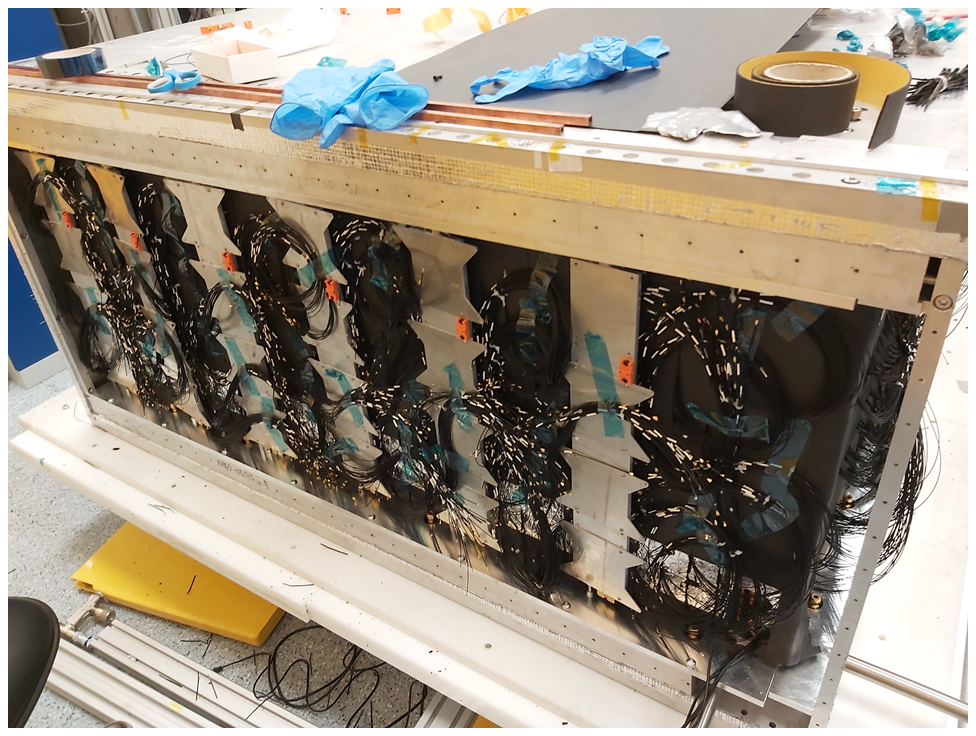
\includegraphics[width=0.8\linewidth]{Chapter3/Figs/Raster/detCon030b_RadiatorWithFins.png}
\captionof{figure}{The radiator on side A with the cooling fins and analogue board holders attached with cables pushed through the insulation and bunched.} 
\label{fig:detCon030b_RadiatorWithFins}
\end{figure}

\begin{figure}[!h]
\centering
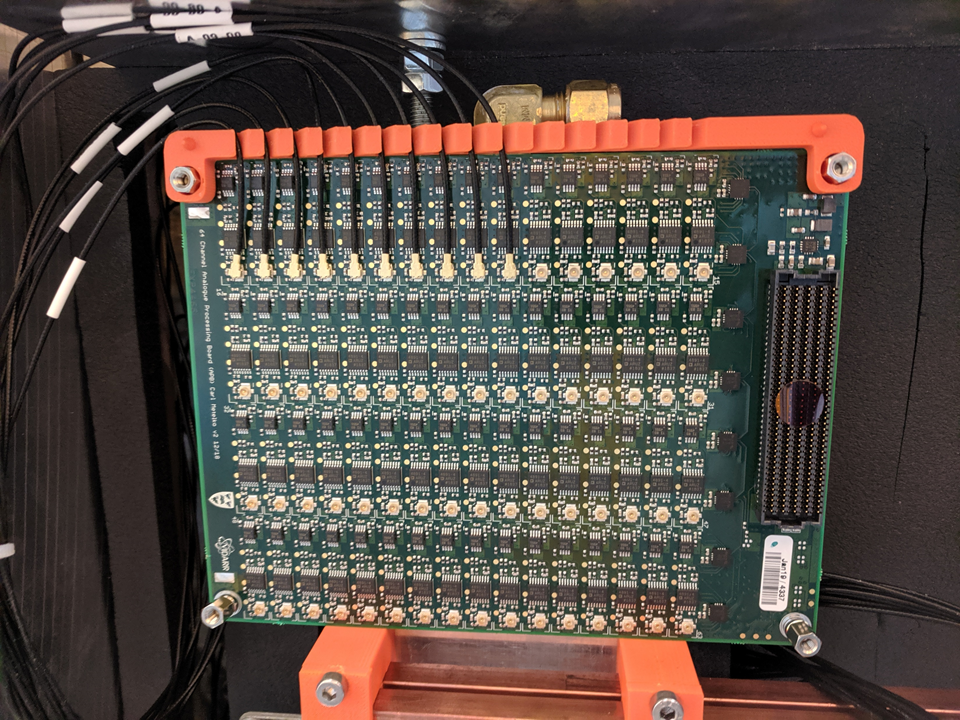
\includegraphics[width=0.8\linewidth]{Chapter3/Figs/Raster/detCon032_ConnectedBoard.png}
\captionof{figure}{An analogue board with some of the cables connected to it. A 3D printed cable ``comb'' is used to align the cables.} 
\label{fig:detCon032_ConnectedBoard}
\end{figure}

The upgraded container was delivered 18$^{th}$ of September 2019 which can be seen in figure  \ref{subFig:detCon037c_ContainerArrives}. But it wasn't until 24$^{th}$ of November 2020 that the detector was placed inside its new container (figure \ref{subFig:detCon039b_PutIn2}). The detector upgrade was not complete at this point and currently remains incomplete this is largely due to the COVID-19 pandemic. The upgrade's progress ceased around the same time as the container arrived during September of 2019 as an issue with electronics was discovered. Currently, this remains unresolved. Due to the issues in the electronics supply chain caused by the COVID-19 crisis and the small size of the VIDARR collaboration obtaining replacement electronics has been impossible up to September of 2021. Though in recent months there has been some movement in obtaining the relevant components. 

\begin{figure}[!h]
\centering
\begin{subfigure}{.5\textwidth}
  \centering
  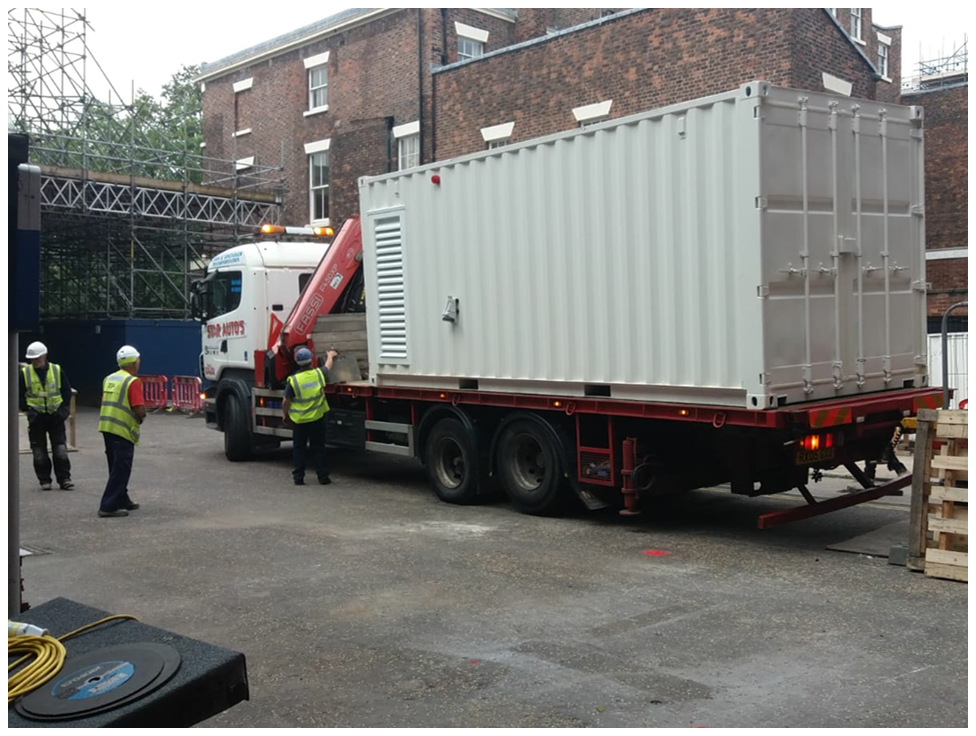
\includegraphics[width=\linewidth]{Chapter3/Figs/Raster/detCon037c_ContainerArrives.png}
  \captionsetup{width=.9\linewidth}
  \caption{The new container arrives at the University of Liverpool.}
  \label{subFig:detCon037c_ContainerArrives}
\end{subfigure}%
\begin{subfigure}{.5\textwidth}
  \centering
  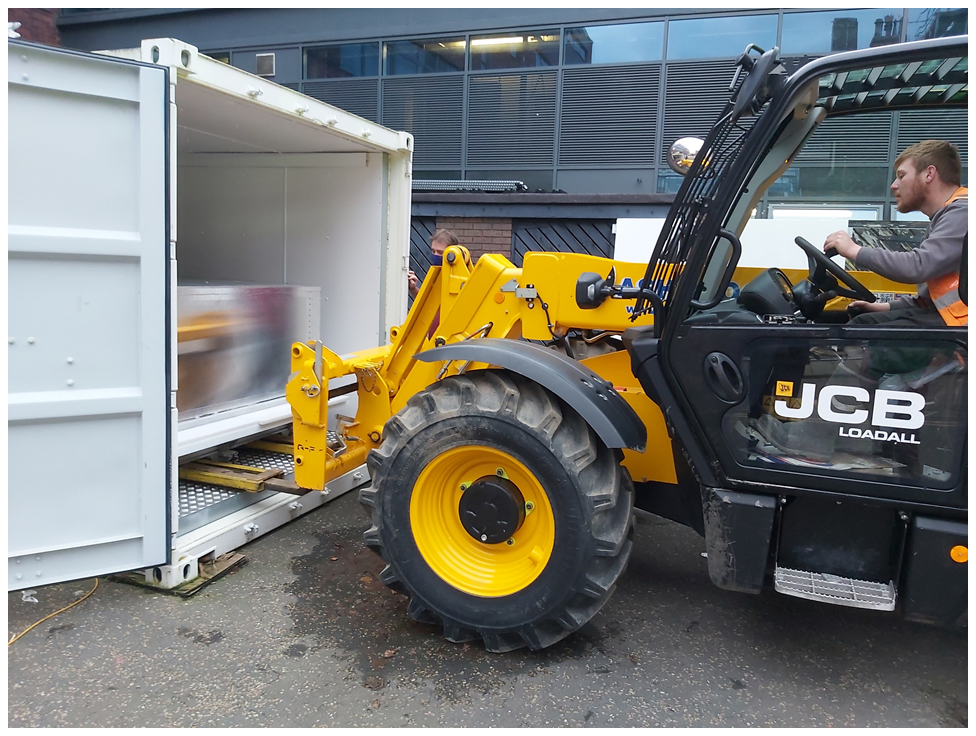
\includegraphics[width=\linewidth]{Chapter3/Figs/Raster/detCon039b_PutIn2.png}
  \captionsetup{width=.9\linewidth}
  \caption{The partially upgraded detector being deposited in the new container.}
  \label{subFig:detCon039b_PutIn2}
\end{subfigure}
\caption{The new container arrives and the partially upgraded detector is deposited inside of it.}
\label{fig:detCon_ContainerArrives_PutIn}
\end{figure}

The upgraded container has much improved airflow when compared to the original. 
In figure  \ref{fig:detCon035b_ContainerAirCon} the air conditioning and improved ventilation system can be seen. The upgraded container should be able to keep the temperature consistent and thus reduce the uncertainties caused by temperature fluctuations. In addition, there has been a significant improvement to computational power with both a new computer rack seen in figure \ref{fig:detCon042b_Rack1}. And a powerful new computer with 64 total threads and 64\,Gb of RAM is seen in figure \ref{fig:detCon044_NewComputer}. Neither of these are currently in the container due to the issues with COVID-19 previously discussed as they are being used to diagnose any issues with the electronics and analyse older data sets.  

\begin{figure}[!h]
\centering
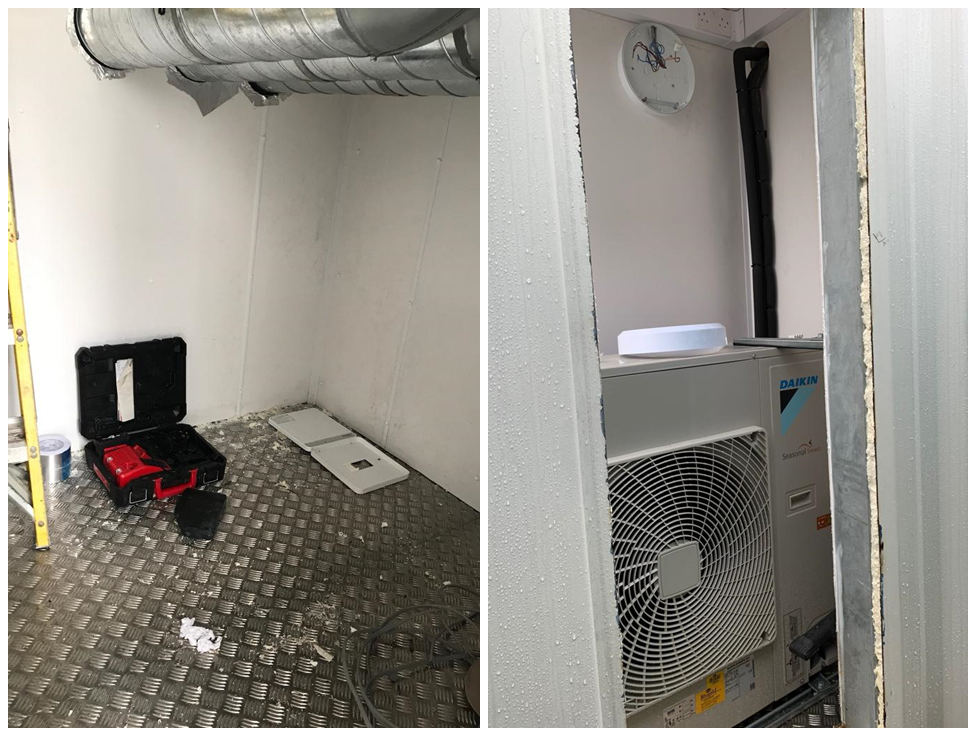
\includegraphics[width=0.7\linewidth]{Chapter3/Figs/Raster/detCon035b_ContainerAirCon.png}
\captionof{figure}{The new container has air conditioning and an air circulatory system to help keep a consistent temperature.} 
\label{fig:detCon035b_ContainerAirCon}
\end{figure}

% \begin{figure}[!h]
% \centering
% 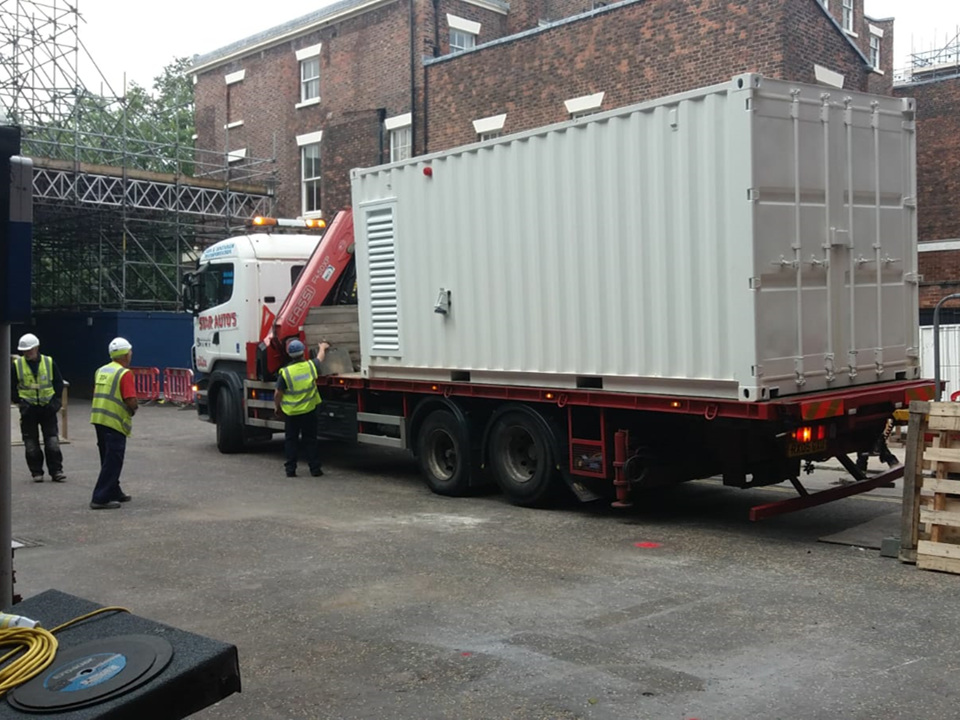
\includegraphics[width=0.8\linewidth]{Chapter3/Figs/Raster/detCon037b_ContainerArrives.png}
% \captionof{figure}{The new container arrives at the University of Liverpool.} 
% \label{fig:detCon037b_ContainerArrives}
% \end{figure}

% \begin{figure}[!h]
% \centering
% 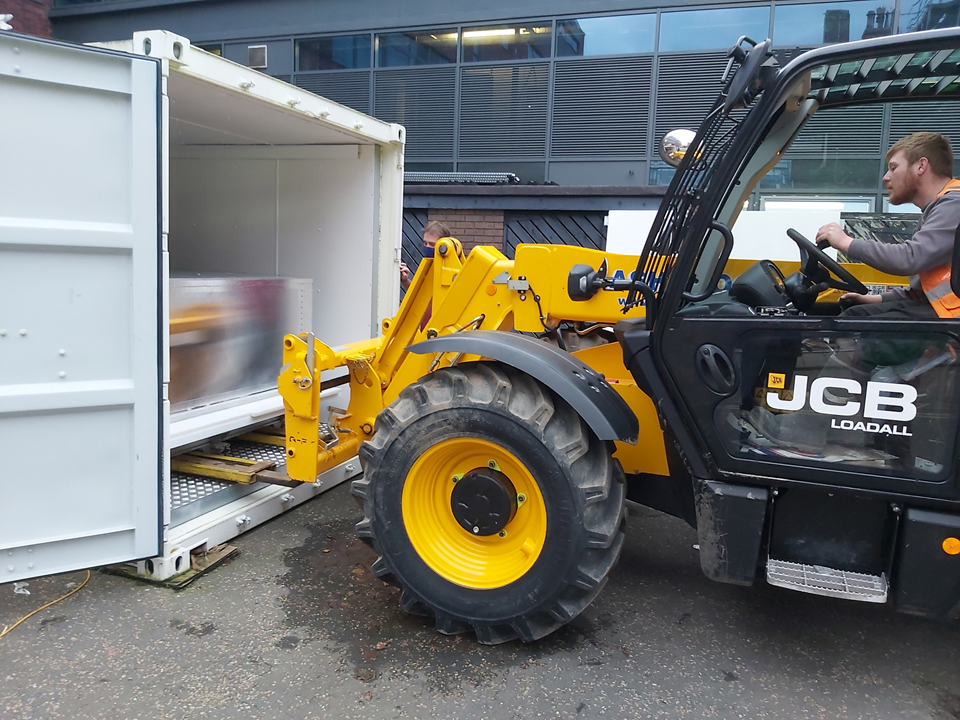
\includegraphics[width=0.8\linewidth]{Chapter3/Figs/Raster/detCon039_PutIn2.png}
% \captionof{figure}{The new detector being placed in the new container. (The upgrade was only partially completed at this time)} 
% \label{fig:detCon039_PutIn2}
% \end{figure}

\begin{figure}[!h]
\centering
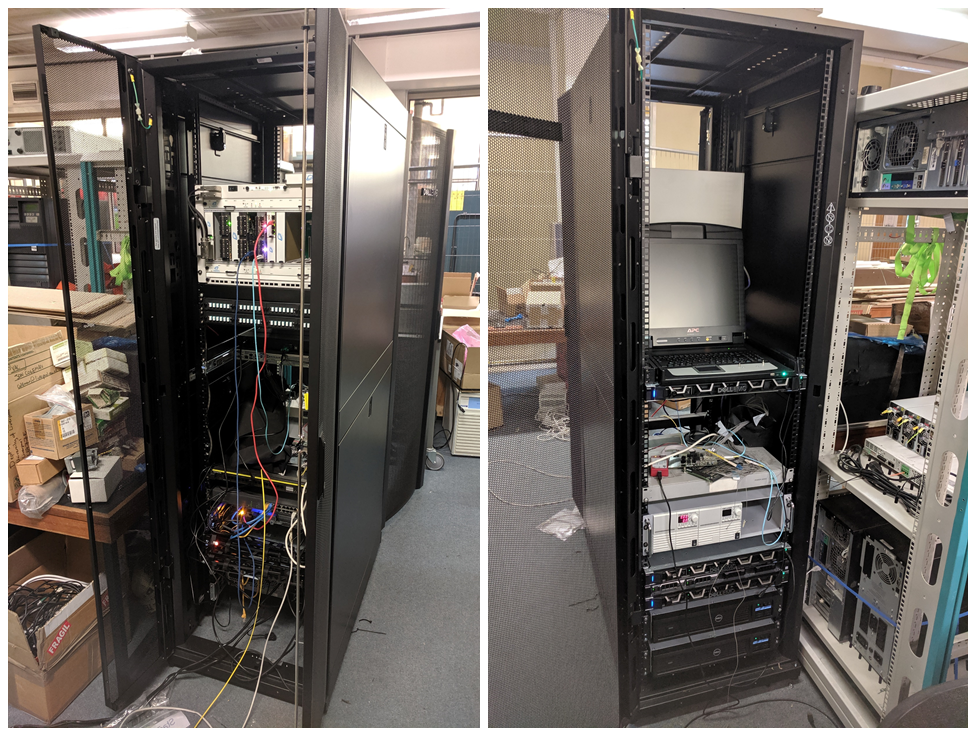
\includegraphics[width=0.7\linewidth]{Chapter3/Figs/Raster/detCon042b_Rack1.png}
\captionof{figure}{The computer rack for the upgraded detector from the back (left) and front (right).} 
\label{fig:detCon042b_Rack1}
\end{figure}

\begin{figure}[!h]
\centering
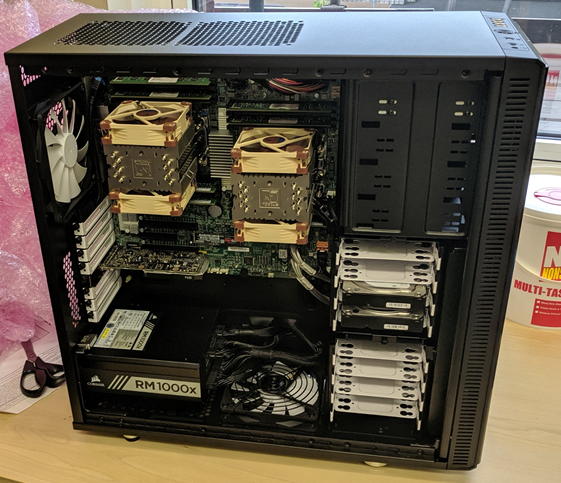
\includegraphics[width=0.8\linewidth]{Chapter3/Figs/Raster/detCon044_NewComputer.png}
\captionof{figure}{The new computer for the upgraded detector. It has two 32 core CPUs and 64\,Gb of Ram.} 
\label{fig:detCon044_NewComputer}
\end{figure}

% \begin{figure}[!h]
% \centering
% 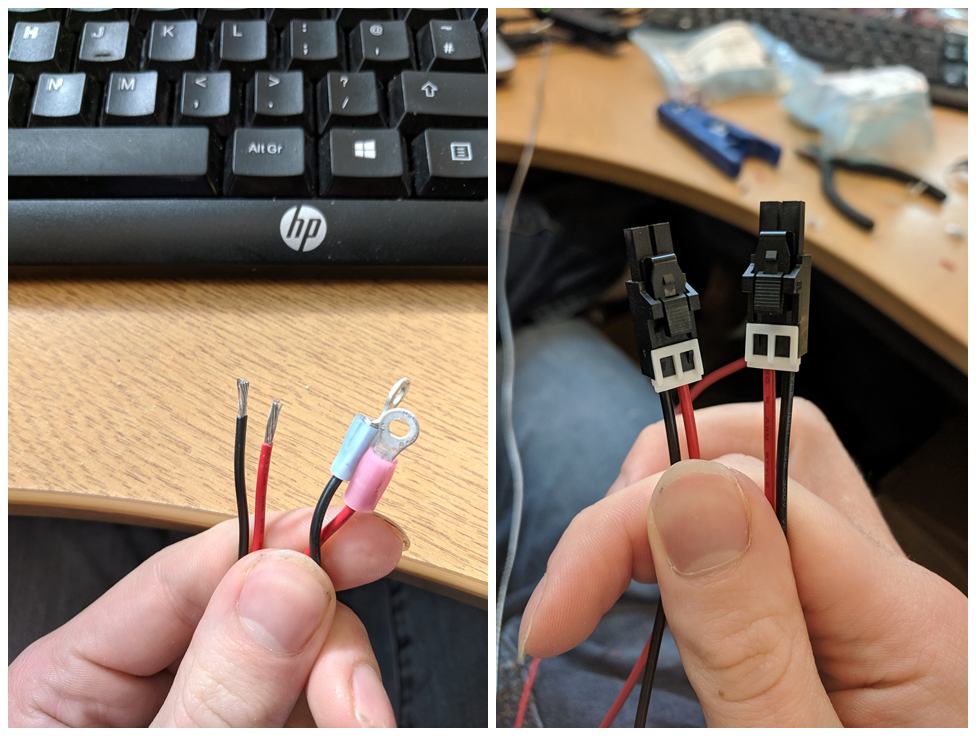
\includegraphics[width=0.7\linewidth]{Chapter3/Figs/Raster/detCon045b_PowerCabels1.png}
% \captionof{figure}{Power cables for the analogue boards that will attach to the central bus bars. \hl{may need to add some finer details remember to check with Carl}} 
% \label{fig:detCon045b_PowerCabels1}
% \end{figure}